\lstset{basicstyle=\footnotesize\sffamily}

Apr\`es un examen des mod\`eles d'architectures et de composants, ce
chapitre est consacr\'e \`a une revue des
th\'eories, techniques et outils relatifs au test fonctionnel de
logiciels en g\'en\'eral et plus particuli\`erement aux m\'ethodes
de g\'en\'eration automatique de tests \`a partir de
sp\'ecifications formelles de comportement sous la forme de
syst\`emes d'\'etats-transitions. 

Nous commencerons cet expos\'e par un certain nombre de
g\'en\'eralit\'es et de d\'efinitions sur le test de logiciels : la profusion de termes a induit une consid\'erable confusion sur
le sens des mots et l'objectif des diff\'erentes techniques \`a la
disposition du testeur. La deuxi\`eme partie de ce chapitre sera
consacr\'ee \`a l'\'etude de la probl\'ematique du test
fonctionnel automatis\'e bas\'e sur un mod\`ele formel qui constitue le c\oe ur
de notre d\'emarche. Nous \'etudierons comment diff\'erents
formalismes d\'efinissent un contexte de test, c'est \`a dire un
cadre formel de validation des r\'esultats du test et comment il est
possible de construire des ensembles de \emph{cas de test}, c'est \`a dire
des \emph{suites de test}, de mani\`ere automatis\'ee. La d\'efinition de
la  notion de conformit\'e d'une implantation donn\'ee par rapport
\`a une sp\'ecification sera bien \'evidemment abord\'ee. Nous terminerons enfin ce chapitre par une
synth\`ese des m\'ethodes de test structurel et une discussion des
probl\'ematiques relatives au test de composants architecturaux.

\section{G\'en\'eralit\'es}

G.Myers dans son ouvrage abondamment
cit\'e\cite{art-soft-test} d\'efinit le test comme suit : 
\begin{quote}
    \og Testing is the process of executing a program with the intent
    of finding errors.~\fg
\end{quote}

Autrement dit, le test est, comme toute activit\'e exp\'erimentale,
 un processus qui pr\'esuppose l'existence d'erreurs et qui a pour
objectif de les trouver. Par cons\'equent, et ce point a \'et\'e
soulign\'e historiquement par E.Dijkstra dans une autre
citation c\'el\`ebre,
\begin{quote}
    \og Testing can show the presence of bugs but never their abscence.\fg
\end{quote}
Le r\'esultat d'un processus de test fini est donc, dans le meilleur des
cas, une forte pr\'esomption d'absence d'erreurs mais jamais une
certitude et de fait un test r\'eussi est un test qui \emph{trouve} une
erreur. Cela ne nous emp\^echera pas par la suite de raisonner en posant
l'hypoth\`ese de l'existence d'un ensemble de tests exhaustif, c'est
\`a dire susceptible de nous fournir une garantie certaine de
correction, mais ce raisonnement servira uniquement de point de
d\'epart th\'eorique pour produire des tests de la mani\`ere la
plus ad\'equate possible.  

L'unit\'e de base du test est le \textbf{cas de test} ou \textbf{test \'elementaire}. Un cas de test,
d'apr\`es \cite{itu-z500}, 
\begin{quote}
    \og [...] pr\'ecise le comportement du testeur dans une
    exp\'erimentation s\'epar\'ee qui teste un aspect de
    l'impl\'ementation sous test [\textsf{IUT} pour \emph{Implementation
    Under Test}] et qui donne lieu \`a une observation et \`a un
    verdict. \fg
\end{quote}
Un ensemble de cas de test constitue une \textbf{suite de tests}.

\subsection{Typologie}

Cette section d\'efinit un certain nombre de termes couramment
utilis\'es dans le domaine du test. Certains d'entre eux recevront une d\'efinition plus
pr\'ecise dans les autres sections de ce chapitre. Le lecteur pourra
se r\'ef\'erer aux ouvrages classiques du domaine d'o\`u sont
tir\'es, parfois paraphras\'es ou l\'eg\'erement
modifi\'es, les termes introduits dans cette section :
\cite{binder,art-soft-test,bb-testing,testlog,itu-z500}. 
 
\subsubsection{Strat\'egie de test}

Une typologie du test peut tout d'abord \^etre faite en fonction de
la strat\'egie de test mise en \oe uvre et des objets manipul\'es
par le processus de test. 
Dans le \textbf{test fonctionnel}, le processus de test
dispose :
\begin{itemize}
  \item d'une \emph{sp\'ecification} du comportement du programme ;
  \item d'un \emph{programme} \`a tester, suppos\'e respecter la
  sp\'ecification.
\end{itemize}
La sp\'ecification est ici utilis\'ee \`a la fois pour d\'efinir
la \emph{suite de test}, c'est \`a dire un ensemble --- fini --- de tests
atomiques, et pour valider le comportement observ\'e du programme
soumis aux tests, jouant ainsi le r\^ole d'\textbf{oracle} de
test. Le test fonctionnel est  aussi appel\'e test \emph{bo\^{\i}te noire},
test \emph{bas\'e sur les mod\`eles}, test \emph{bas\'e sur les
sp\'ecifications}, test de \emph{conformit\'e}, test \emph{comportemental}

Lorsque la sp\'ecification d\'ecrit des propri\'et\'es non
applicatives du logiciel, par exemple des temps de r\'eponse, des
taux de transferts, la tol\'erance aux pannes, la capacit\'e de
reprise sur erreur, la mont\'ee en charge, on parlera de \textbf{test 
non-fonctionnel} ou de \emph{test de qualit\'e de service}. La distinction entre une propri\'et\'e applicative et une
propri\'et\'e de qualit\'e de service est purement arbitraire comme
l'est la s\'eparation entre exigences fonctionnelles et exigences
techniques.  Elle d\'epend g\'en\'eralement du processus m\'etier
mat\'erialis\'e par le logiciel : le fonctionnel d'un d\'eveloppeur
de \textsf{SGBDR} ou de logiciels de routage est le non-fonctionnel
d'un syst\`eme d'information d'entreprise.

On oppose g\'en\'eralement au test fonctionnel le \textbf{test
  structurel} dit aussi test \emph{bo\^{\i}te blanche}, test \emph{bo\^{\i}te de verre},
test \emph{bas\'e sur le code}. Dans le test
structurel, le processus du test dispose du programme \`a tester et
de son \emph{code source}, ce dernier servant \`a la
g\'en\'eration des cas de test, dans l'optique de produire une suite
de test ad\'equate pour un certain objectif de couverture (voir
section \ref{sec:test-structurel}). Le test structurel est \`a notre avis une option
suppl\'ementaire au test fonctionnel, c'est \`a dire un moyen de
compl\'eter l'information donn\'ee par la sp\'ecification avec des
informations contenues dans le code du logiciel test\'e, dans le but
  d'am\'eliorer la pertinence des r\'esultats obtenus par le test. 

Pour \'eviter la confusion avec la terminologie surcharg\'ee du mot mod\`ele, nous
d\'esignerons l'ensemble des \'el\'ements \`a la disposition du
processus de test pour construire une suite de test par le terme
d'\textbf{analogue de test} : documentation, sp\'ecifications formelles
ou non, exigences, code source, assembleur peuvent tous faire partie
de l'analogue de test et \^etre utilis\'es pour construire des cas
de test.

L'\textbf{objectif de test} d\'efinit la mani\`ere dont vont \^etre
produits les cas de test. \'Etant entendu qu'il est impossible,
hormis les cas les plus triviaux, de tester exhaustivement une
entit\'e logicielle, la fixation d'un objectif de test permet de
s\'electionner les cas de test parmi l'ensemble de tous les cas de
test possibles. Un autre terme d\'esignant le m\^eme concept est
celui de  \textbf{crit\`ere de test}. Le terme anglais de \emph{test
  purpose}, aussi traduit par objectif de test, est un cas particulier
de l'objectif de test au sens d\'efini ici : une s\'election
restreinte dans l'ensemble des comportements de l'entit\'e \`a
tester. La
d\'efinition d'un objectif d\'epend \'evidemment des \'el\'ements \`a la disposition du
testeur. 

Le terme de \textbf{couverture} d\'esigne une famille de
crit\`eres dans laquelle on cherche \`a obtenir une suite de
tests permettant de couvrir une certaine fraction de l'\emph{analogue
  de test}. Dans son acception la plus courante, la couverture est
celle du code de l'implantation sous test dans le cadre du test structurel. 

Des crit\`eres de test peuvent aussi \^etre
\emph{statistiques}, en liaison avec la notion de fiabilit\'e statistique du
logiciel et de \emph{profil op\'erationnel} d'utilisation, ou des
crit\`eres \emph{heuristiques} --- on parlera aussi d'\emph{hypoth\`eses de
  test} --- li\'es \`a un certain \emph{mod\`ele de d\'efaut} :
par exemple, le fait de s\'electionner parmi un ensemble de valeurs
possibles pour les param\`etres d'une fonction des valeurs limites
est un crit\`ere heuristique courant. 

Un objectif pour le processus de test peut \^etre constitu\'e d'une
combinaison quelconque d'un ensemble de sous-objectifs et peut servir
soit dans le cadre d'un processus de g\'en\'eration automatique,
soit dans un processus de production manuelle des cas de tests. Le
probl\`eme principal consiste \`a s'assurer que
l'objectif a bien \'et\'e atteint.

Enfin, une strat\'egie de test est toujours li\'ee \`a un \textbf{mod\`ele
de d\'efaut}, implicite ou explicite, c'est \`a dire un ensemble
d'hypoth\`eses sur les d\'efauts pr\'esents dans l'implantation test\'ee : on ne peut
g\'en\'eralement d\'etecter que les pannes que l'on cherche. Ce
mod\`ele de d\'efaut d\'epend  de l'analogue de test. 

\subsubsection{Granularit\'e}

Une autre dimension donnant lieu \`a une grande variation de
terminologie concerne la \emph{granularit\'e} des entit\'es que l'on
souhaite tester. La granularit\'e a un impact \'evident sur la
strat\'egie de test puisque selon les cas, le processus de test aura
\`a sa disposition diff\'erentes informations pour construire sa
suite de tests et \'evaluer le r\'esultat.

Le \textbf{test d'acceptation} appel\'e aussi plus commun\'ement \emph{test de
recette} ou simplement \emph{recette} vise \`a valider un syst\`eme
complet du point de vue de l'\emph{utilisateur} du syst\`eme. C'est
g\'en\'eralement la derni\`ere phase du d\'eveloppement d'un
logiciel avant sa \emph{livraison} et  le
d\'emarrage, si n\'ecessaire, d'une nouvelle it\'eration du cycle de
d\'eveloppement. \'Etant r\'ealis\'e du point de vue de
l'utilisateur, le test d'acceptation va chercher \`a exercer
l'ensemble des fonctionnalit\'es du logiciel en situation de
production. Les \emph{jeux et plans de tests} sont d\'evelopp\'es
\`a partir des exigences du cahier des charges, compl\'et\'ees de la
connaissance des utilisateurs du syst\`eme agissant comme testeurs.

Le \textbf{test syst\`eme} est similaire dans sa port\'ee au test
d'acceptation : l'implantation sous test ---  \textsf{IUT}, \emph{Implementation
  Under Test} --- est le syst\`eme complet et le processus va
chercher \`a valider son comportement par rapport aux exigences
exprim\'ees par l'utilisateur et transcrites dans l'analyse et la
conception. Le test syst\`eme est aussi
appel\'e test \emph{bas\'e sur les exigences} --- \emph{requirements
  based testing}. 

Le terme de \textbf{test unitaire} est applicable \`a diff\'erents
niveaux de granularit\'e : il consiste \`a tester en isolement une
entit\'e sp\'ecifique susceptible \'eventuellement d'\^etre
compos\'ee ou int\'egr\'ee par la suite dans une entit\'e plus
vaste. Le point important dans le test unitaire est la notion
d'\emph{isolement} : l'\textsf{IUT} est test\'e en dehors de toute interaction
avec d'autres entit\'es du syst\`eme  ce qui suppose
d'\^etre capable : 
\begin{enumerate}
  \item de l'\emph{ex\'ecuter} de mani\`ere autonome ;
  \item de \emph{simuler} sous
    contr\^ole du testeur l'environnement n\'ecessaire \`a son bon fonctionnement .
\end{enumerate}

Le \textbf{test d'int\'egration} a pour
objets un ensemble d'entit\'es logiquement li\'ees et dont on
cherche \`a v\'erifier qu'elles peuvent coop\'erer. Les entit\'es concern\'ees peuvent \^etre aussi simples que
des fonctions ou m\'ethodes  d'une classe, une grappe
d'objets formant un tout coh\'erent ou un ensemble de
sous-syst\`emes formant un syst\`eme plus complet. Le test
d'int\'egration peut \^etre vu comme une phase pr\'eparatoire
au test unitaire d'un niveau de granularit\'e plus \'elev\'e.

Le \textbf{test de non-r\'egression} permet d'une part de s'assurer du maintien
des fonctionnalit\'es d'un IUT entre deux versions, d'autre part de
v\'erifier que des erreurs corrig\'ees dans une version $n$ ne
r\'eapparaissent pas dans une version $n+1$. Pour chaque erreur
d\'etect\'ee par la recette ou le test syst\`eme, un cas de test
t\'emoin est produit qui va enrichir la suite de tests de
non-r\'egression.

\subsection{Ex\'ecution du test}

Le test est une activit\'e de v\'erification \emph{dynamique} d'un
objet logiciel : il suppose l'\emph{ex\'ecution} du logiciel et
l'observation de son comportement. Cette ex\'ecution produit un r\'esultat qui
d\'epend des fonctionnalit\'es de l'entit\'e logicielle test\'ee :
une fonction produit une valeur \`a partir de param\`etres
d'entr\'ee, un objet change d'\'etat en fonction des m\'ethodes qui
sont invoqu\'ees, un syst\`eme de gestion  transforme des
donn\'ees stock\'ees dans une base de donn\'ees en fonction des
actions r\'ealis\'ees par un utilisateur, un syst\`eme de
pilotage d'une cha\^{\i}ne de production \'emet des commandes en
fonction de la r\'eception de signaux de son environnement, ...

La conclusion d'un cas de test est donc le r\'esultat de la comparaison
entre le comportement \emph{observ\'e} de l'objet test\'e et le
comportement \emph{attendu} qui est partie int\'egrante de la
d\'efinition d'un cas de test. Cette comparaison produit donc un
\textbf{verdict de test} qui peut \^etre :
\begin{itemize}
  \item un \textbf{succ\`es} lorsque le comportement observ\'e est
    \'egal, quel que soit le sens de \emph{\'egal} dans le contexte choisi,
    au comportement attendu ;
  \item un \textbf{\'echec} lorsque les comportements observ\'e et
    attendu divergent. 
\end{itemize}
En anglais, on parlera dans ce dernier cas de \emph{failure}, terme
que l'on peut aussi traduire par \emph{panne}. Il ne faut pas
confondre une \emph{panne} avec un \emph{d\'efaut} --- \emph{fault}
en anglais. Un d\'efaut est un \'el\'ement de l'objet test\'e \`a l'origine de l'\'echec ou
de la panne. Une \emph{erreur} est une action ou une inaction
humaine ayant provoqu\'e l'introduction du d\'efaut et donc
indirectement la panne. Un m\^eme d\'efaut peut \^etre \`a l'origine de
plusieurs pannes  et inversement une panne peut \^etre caus\'ee par
la conjonction d'un ensemble de d\'efauts. Le cas peut m\^eme
exister de d\'efauts qui se corrigent entre eux pour \emph{masquer} une panne.
Le \emph{d\'everminage} --- \emph{debugging} en anglais  --- est
l'activit\'e consistant \`a identifier les d\'efauts et corriger
les erreurs ayant entra\^{\i}n\'e un \'echec lors du test.

Certains auteurs et la norme \cite{itu-z500} d\'efinissent aussi comme r\'esultat possible du
test le r\'esultat \emph{non-concluant} : aucun \'echec n'a
\'et\'e constat\'e mais il est n\'ecessaire de poursuivre
l'ex\'ecution du test pour valider le r\'esultat. Cette notion
renvoie \`a la d\'efinition d'un objectif de test. Un test ou un
ensemble de tests peuvent \^etre consid\'er\'es comme
non-concluants tant que l'objectif de test n'est pas atteint. Ce type
de verdict  n'est
pas \`a notre avis directement li\'e \`a l'ex\'ecution
d'\emph{un} test. 
Un r\'esultat non-concluant peut aussi survenir
lorsque le comportement de l'objet test\'e est inobservable, c'est
\`a dire que l'on est incapable de conclure sur le r\'esultat du
test du fait de l'absence de r\'esultat observ\'e.

Ceci nous am\`ene naturellement aux notions d'\textbf{observabilit\'e}
et de \textbf{contr\^olabilit\'e} de l'\emph{IUT} qui d\'efinissent
sa \textbf{testabilit\'e}. Un \textsf{IUT} est \emph{observable} si le
r\'esultat \emph{observ\'e} d'\emph{un} test sur cet \textsf{IUT} d\'epend uniquement
de ce test. Il est \emph{contr\^olable} si \emph{tous} les r\'esultats
attendus peuvent \^etre observ\'es par l'ex\'ecution d'un test. Ces
concepts sont introduits dans \cite{freedman-testability} pour les programmes
proc\'eduraux et g\'en\'eralis\'es dans \cite{formspectest}. Il
s'agit ici de propri\'et\'es de l'\textsf{IUT} --- et indirectement de la
sp\'ecification \`a partir de laquelle l'\textsf{IUT} a \'et\'e
d\'evelopp\'e --- qui peuvent avoir de toute \'evidence un grand
impact sur la capacit\'e du test \`a r\'ev\'eler des pannes.

La proc\'edure de d\'ecision effectuant la comparaison entre r\'esultat attendu et r\'esultat observ\'e est
appel\'ee \textbf{oracle de test} et sa construction correcte est
bien \'evidemment un point essentiel du processus de test. Cet oracle
est d\'eduit, manuellement ou automatiquement, de l'\emph{analogue de
  test}. Sa correction suppose, comme nous l'avons vu, que cet
analogue soit lui m\^eme \emph{testable}, c'est \`a dire observable et
contr\^olable. Le probl\`eme de l'oracle n'est pas un probl\`eme
trivial mais dans le cas o\`u l'analogue utilis\'e pour le test est
une sp\'ecification formelle, ce probl\`eme est normalement
r\'esolu par la s\'emantique propre au syst\`eme formel utilis\'e.

\subsection{Synth\`ese}

La figure \ref{fig-activite-test} repr\'esente sous la forme d'un
diagramme d'activit\'e UML les interactions entre les diff\'erentes
entit\'es menant \`a la d\'efinition et l'ex\'ecution d'un
processus de test. Ce sch\'ema met en avant un point \`a notre avis
crucial du processus de test : l'impact que celui-ci peut avoir
sur la conception --- l'analogue dans le sch\'ema. D'une
part, comme nous l'avons vu dans la pr\'ec\'edente section, la
testabilit\'e d'une entit\'e logicielle d\'epend fortement de
celle de sa sp\'ecification au sens le plus large. Par
cons\'equent le fait de mettre en place un processus de test suppose
que l'on ait v\'erifi\'e cette derni\`ere ou que l'on puisse la
corriger en fonction des r\'esultats du processus de test. D'autre
part, et de mani\`ere assez \'evidente, l'\'echec d'un test compte
tenu des diff\'erentes entit\'es qui entrent en jeu dans sa
construction et son ex\'ecution peut signifier que :
\begin{itemize}
  \item soit l'implantation test\'ee pr\'esente un d\'efaut, ce qui
  est le cas le plus \og favorable \fg  ;
\item soit l'analogue pr\'esente un d\'efaut : par hypoth\`ese, le
  processus de d\'eveloppement est une activit\'e humaine tandis
  que, dans le cas qui nous int\'eresse, le processus de construction
  des tests est une activit\'e automatis\'ee. Il est donc possible
  que des erreurs dans l'analogue ne soient pas conserv\'ees
  dans l'implantation alors qu'elles le seront dans la suite de tests ;
\item soit la  suite de tests elle-m\^eme pr\'esente un
  d\'efaut. Cette possibilit\'e est supprim\'ee toujours par
  hypoth\`ese d'une transformation automatis\'ee --- et fiable --- de
  l'analogue en suite de test.
\end{itemize}

\begin{figure}{htbp}
    \centering
    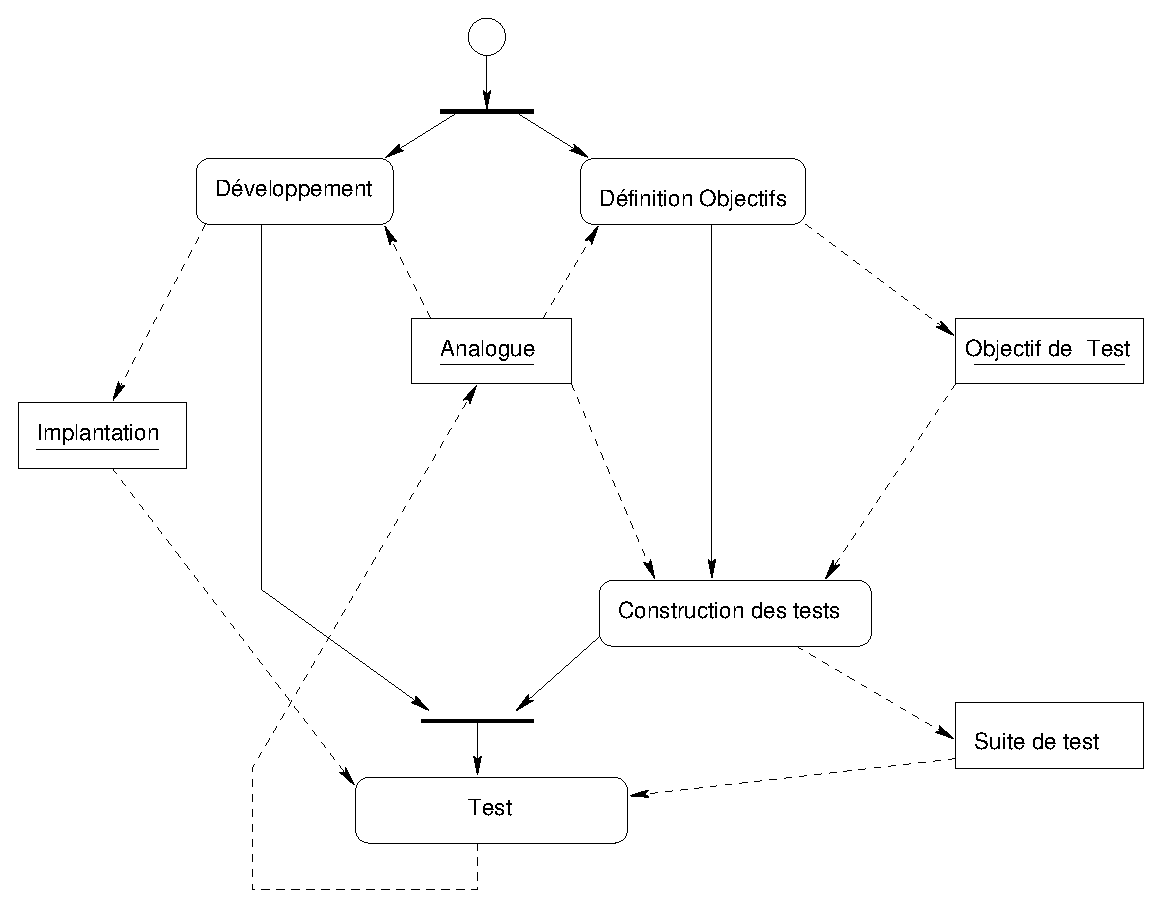
\includegraphics[width=.6\textwidth]{figures/fig-activite-test.eps}
    \caption{Activit\'e de test}
    \label{fig-activite-test}
\end{figure}

La figure \ref{fig-processtest} est une vue plus pr\'ecise de
l'activit\'e de test proprement dite, applicable \`a diff\'erents niveaux de
granularit\'e. Le processus requiert tout d'abord la validation des
tests d'int\'egration des diff\'erentes entit\'es int\'egr\'ees
dans l'\textsf{IUT}. On suppose par ailleurs que leur testabilit\'e est
contr\^ol\'ee en amont du processus. La conception des tests
d\'epend, nous l'avons vu, de l'analogue et de l'objectif fix\'e, le
premier \'etant utilis\'e par ailleurs pour construire
l'\emph{environnement de test} ou \emph{contexte de test}, c'est \`a
dire la simulation de l'ensemble des ressources dont d\'epend
l'\textsf{IUT}. Le processus d'ex\'ecution produit un verdict : si c'est un
\'echec, alors l'\textsf{IUT} contient un ou plusieurs d\'efauts qu'il est
n\'ecessaire de corriger avant de retester ; si c'est un succ\`es,
il est n\'ecessaire alors de v\'erifier que l'objectif de test est
bien atteint. Notons que dans un processus automatis\'e, les suites
de test \'etant produites  \`a partir de l'objectif de test, cette
v\'erification est imm\'ediate et toujours r\'eussie.

\begin{figure}[htbp]
    \centering
    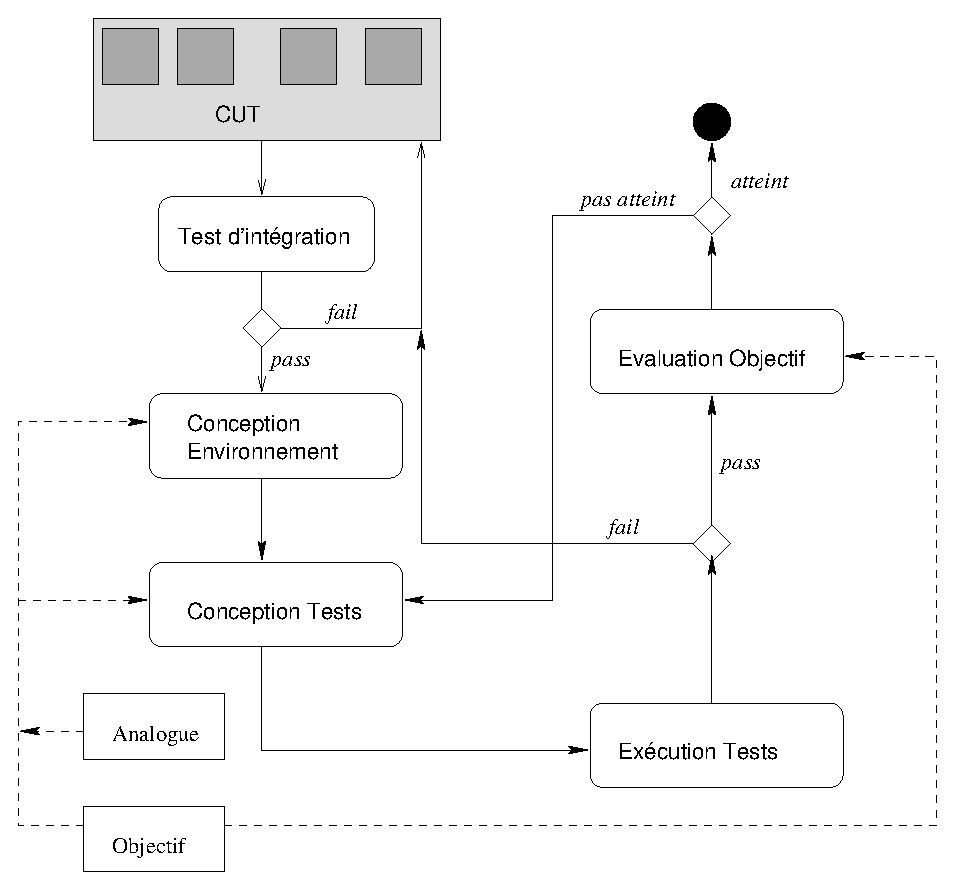
\includegraphics[width=.6\textwidth]{figures/fig-processtest.eps}
    \caption{Activit\'e de test (d\'etail)}
    \label{fig-processtest}
\end{figure}

\section{Test de conformit\'e}

Nous avons \`a la section pr\'ec\'edente fix\'e de mani\`ere
informelle la terminologie parfois confuse que l'on retrouve dans tout
ou partie des travaux sur le test. Nous avons par ailleurs identifi\'e un processus
g\'en\'eral de test unitaire prenant en compte de mani\`ere
abstraite l'ensemble des facteurs conduisant \`a la r\'ealisation
effective d'un processus de test. Il n'est clairement pas question de
passer en revue l'ensemble du domaine extr\^emement riche que
constitue le test de logiciel et nous allons donc nous attacher ici
\`a en d\'etailler la fraction qui nous int\'eresse
particuli\`erement, c'est \`a dire le test bas\'e sur des
\emph{sp\'ecifications formelles comportementales} : machines
d'\'etats finis, syst\`emes de transition, machines abstraites.

Ces travaux sont issus pour beaucoup de la probl\'ematique du test de
protocole de communication. De ce fait leur applicabilit\'e au test
de composants logiciels tels que nous les avons d\'efinis dans les
chapitres pr\'ec\'edent est presqu'imm\'ediate, les architectures de test \'etant fortement similaire. D'un point de vue
th\'eorique, ces travaux sont reli\'es d'une part au probl\`eme de
l'\'equivalence s\'emantique de processus mod\'elis\'es comme des
syst\`emes de transitions, et d'autre part \`a des recherches  sur
l'identification  de machines de 
\textsc{Moore} et plus g\'en\'eralement de transducteurs et  d'automates.

Nous effectuerons toutefois une incursion dans une autre famille de
test, le test bas\'e sur des sp\'ecifications alg\'ebriques, dans
la mesure o\`u certains travaux sur cette cat\'egorie de formalismes
ont produit des concepts pertinents pour le test de conformit\'e de
syst\`emes de transitions.

\subsection{Test alg\'ebrique}

Dans \cite{gaudel} sont  pos\'ees les bases d'une th\'eorie du
test  appliqu\'ee aux sp\'ecifications alg\'ebriques. Cette th\'eorie
est d\'evelopp\'ee dans \cite{thmarre} et par la suite reprise
notamment dans \cite{thspectest,formspectest,reqtottest,testsel,testiodata}.

On cherche ici \`a formaliser des notions
plut\^ot floues que sont la testabilit\'e, la validit\'e d'un test,
la conformit\'e, les hypoth\`eses n\'ecessaires au test. L'id\'ee
principale consiste \`a partir d'une \emph{suite de tests} exhaustive
 pour laquelle, sous une \emph{hypoth\`ese
  de testabilit\'e} de l'implantation consid\'er\'ee, on a
l'assurance que si l'implantation passe la suite de tests, elle est
conforme. Cette suite de tests \'etant g\'en\'eralement
impraticable, elle va \^etre raffin\'ee par applications successives
d'\emph{hypoth\`eses de test}, non-biais\'ees (saines) et
valides, qui permettent d'en r\'eduire la taille. Le processus s'arr\^ete lorsque l'on atteint une suite de tests
acceptable. 

Les deux types d'hypoth\`eses principales sont d\'enomm\'ees
\emph{hypoth\`ese de r\'egularit\'e} et \emph{hypoth\`ese
  d'uniformit\'e}\cite{gaudel}, elles formalisent des pratiques courantes du test
telles que le test de partitionnement, le test aux limites, la
s\'election de profondeurs de boucles ou de r\'ecursions,
... \cite{thphalippou} introduit d'autres hypoth\`eses
telles l'\emph{\'equit\'e} ou l'\emph{ind\'ependance} qui
permettent de g\'erer les probl\`emes li\'es au non-d\'eterminisme
et au parall\'elisme. 

Le couple form\'e des hypoth\`eses de test et
d'une suite de tests r\'eduite issue de l'application des
hypoth\`eses  \`a la
suite de tests exhaustive doit maintenir deux propri\'et\'es :
\begin{enumerate}
  \item il doit \^etre \emph{valide} : si l'implantation
  passe la suite de tests r\'eduite, alors elle passerait la suite de tests
  exhaustive ;
\item il doit \^etre \emph{non-biais\'e} : si
  l'implantation passe  la suite de tests exhaustive, alors elle
  passera la suite de tests r\'eduite.
\end{enumerate}
En d'autres termes, une suite de tests doit accepter toutes
les implantations  correctes et ne  pas accepter les implantations
incorrectes.

Dans \cite{formspectest}, \`a la
notion d'ensemble de test \emph{exhaustif} telle que 
d\'efinie pr\'ec\'edemment s'ajoute la notion d'ensemble complet
d\'efinie comme une suite de tests non-biais\'ee et \emph{maximale}
 : toute autre  suite de tests a un pouvoir de d\'etection plus
faible. Un point important de l'article est qu'un ensemble complet
n'est pas n\'ecessairement exhaustif et qu'il n'existe  pas
n\'ecessairement d'ensemble exhaustif pour un programme donn\'e dans
un certain cadre d'observations. Si certaines
propri\'et\'es du programme test\'e ne sont pas
observables, elles ne pourront \^etre v\'erifi\'ees par le test. Un
programme sera donc consid\'er\'e comme \emph{partiellement correct}
s'il est valide par rapport \`a une suite de tests compl\`ete.

Cette formalisation g\'en\'erale du test est reprise par ailleurs
dans la norme \textsf{IUT Z.500}\cite{itu-z500}, \og Cadre g\'en\'eral des
m\'ethodes formelles appliqu\'ees au test de conformit\'e \fg.

\subsection{Test de Machines \`a \'Etats Finis (\textsf{FSM})}

Une \emph{machine d'\'etat fini} ou \textsf{FSM} --- \emph{Finite
State Machine} --- est un n-uplet $(Q,I,O,q_0,\lambda,\delta)$
avec
\begin{itemize}
  \item $Q$ un ensemble fini d'\'etats ;
  \item $q_0 \in Q$ un \'etat initial distingu\'e ;
  \item $I$ et $O$ des alphabets finis d'\emph{entr\'ee} et de
  \emph{sortie} ;
\item $\lambda : Q\times{}I \rightarrow O^*$ la fonction partielle de sortie ;
\item $\delta : Q\times{}I \rightarrow Q$ la fonction partielle de transition.
\end{itemize}
Un \textsf{FSM} est aussi appel\'e
\emph{transducteur s\'equentiel}\cite{berstel,sakarovitch} et calcule
une  fonction rationnelle transformant un langage d'entr\'ee inclus dans $I^*$ en un 
langage de sortie inclus dans $O^*$. 

\'Etant donn\'ees une machine $A$ dont la structure est connue et
une machine $M$ dont la structure est inconnue mais dont les alphabets
sont suppos\'es identiques \`a ceux de $A$, le  \emph{test
de conformit\'e} de \textsf{FSM} consiste \`a d\'eterminer si les
deux machines calculent la m\^eme fonction en examinant les sorties
produites par $M$ pour un ensemble de mots d'entr\'ees, les
s\'equences de test.

Dans le cas g\'en\'eral o\`u $\lambda$ et $\delta$ sont des
fonctions partielles, on
distinguera\cite{sidhu-study-fsmtest} des s\'equences de test de
\emph{conformit\'e faible}, qui v\'erifient l'\'equivalence de sortie pour
les seules entr\'ees sp\'ecifi\'ees ; et des s\'equences de
test de \emph{conformit\'e forte} g\'en\'er\'ees \`a partir d'une
compl\'etion de la sp\'ecification par des transitions sans sortie
pour les lettres non sp\'ecifi\'ees dans chaque \'etat. 

Un certain nombre d'hypoth\`eses sur $M$ et de contraintes sur $A$
sont g\'en\'eralement pos\'ees pour permettre la construction
effective de s\'equences de test : minimalit\'e et/ou
d\'eterminisme de $A$, bornage du nombre d'\'etats de $M$,
correspondance des alphabets, d\'eterminisme de $M$, ...

Un tel ensemble de  \emph{s\'equences de 
v\'erification} produit un r\'esultat certain et bien \'evidemment,
hormis les cas les plus triviaux, sa construction est ardue. On
trouvera dans \cite{lee96principles} les complexit\'es de cette
construction en fonction des caract\'eristiques de $A$ : existence ou non de \emph{reset}, de \emph{s\'equences
  distinguantes}, ... Nous donnons ci-dessous quelques m\'ethodes
classiques --- ou moins classiques --- de
g\'en\'eration  de s\'equences de tests pour les \textsf{FSM}. 

Le probl\`eme de
l'\'equivalence de \textsf{FSM} remonte au moins aux travaux de Moore dans
\cite{moore-gedanken} : \'etant donn\'e une machine de Moore ---
l'implantation --- peut on \`a l'aide d'exp\'erimentations, c'est
\`a dire de s\'equences de l'alphabet d'entr\'ee, d\'eduire des
sorties produites par la machine test\'ee l'\emph{\'etat initial} de
celle-ci ? Plus g\'en\'eralement, peut-on toujours \emph{distinguer} deux machines
\`a l'aide de s\'equences de test ? La r\'eponse dans le cas
g\'en\'eral est \emph{non} : la propri\'et\'e de
distinguabilit\'e est ind\'ecidable pour une machine
arbitraire. Elle est d\'ecidable dans le cas de machines minimales de
taille born\'ee et l'on obtient m\^eme directement une borne
sup\'erieure sur la taille des suites de tests n\'ecessaires pour
distinguer deux machines donn\'ees --- \emph{ie.} une implantation inconnue
mais suppos\'ee de taille born\'ee, d\'eterministe et totalement
connexe et une sp\'ecification connue.

\subsection{S\'election des cas de test dans les \textsf{FSM} d\'eterministes}

\begin{figure}
\epsfig{width=.70\textwidth,file=figures/fig-sample-fsm.eps}
\caption{Sp\'ecification  d'un \textsf{FSM}}
\label{fig-sample-fsm}
\end{figure}

Nous pr\'esentons ici quelques m\'ethodes classiques appliqu\'ees
au test de \textsf{FSM} d\'eterministes. Cette probl\'ematique est
historiquement importante et th\'eoriquement int\'eressante, m\^eme
si en pratique son applicabilit\'e \`a la g\'en\'eration de tests
pour des probl\`emes r\'eels est faible de par la complexit\'e des
algorithmes et surtout la taille exponentielle des suites de tests
g\'en\'er\'ees. D'apr\`es \cite{lai-prototest-survey}, il semble
que seule la m\'ethode \textsf{UIO} ait \'et\'e appliqu\'ee \`a
une \'echelle industrielle dans le cadre du test de logiciels  de
t\'el\'ecommunications. 
Pour illustrer ces diff\'erentes m\'ethodes, nous utiliserons
la sp\'ecification pr\'esent\'ee dans la figure
\ref{fig-sample-fsm}, exemple tir\'e de \cite{sidhu-study-fsmtest}.

\subsubsection{Le \emph{tour de transition}}

Dans le cas d'un \textsf{FSM} fortement connexe, le tour de transition consiste
\`a construire une s\'equence de test unique par parcours de
l'ensemble des transitions du graphe du \textsf{FSM}. Cette construction peut
\^etre faite soit analytiquement par un parcours du graphe, soit par
un parcours al\'eatoire suivi d'une \'elimination des
sous-s\'equences redondantes. 

\subsubsection{La m\'ethode \textsf{W}}
\label{sec:la-methode-w}

La m\'ethode \textsf{W} a \'et\'e introduite dans \cite{chow-w-method} et
depuis abondamment reprise comme bases d'autres m\'ethodes ou
cit\'ee comme r\'ef\'erence. Le
principe de cette m\'ethode consiste \`a construire un ensemble de
s\'equences de tests, c'est \`a dire de mots appartenant \`a
l'alphabet d'entr\'ee  du \textsf{FSM} sp\'ecifi\'e, permettant de
v\'erifier pour chaque \'etat $q$, d'une part l'existence de cet
\'etat dans l'implantation sous test, d'autre part la conformit\'e
des sorties produites \`a partir de cet \'etat.

Cette m\'ethode est bas\'ee sur la construction d'un ensemble de
s\'equences \emph{caract\'eristiques} ou \emph{ensemble de distinction}, appel\'e ensemble $W$, qui
est tel que tous les \'etats du \textsf{FSM} produisent \`a partir
de $W$ un ensemble de s\'equences de sorties diff\'erent et sont
donc distinguables les uns des autres. Elle utilise aussi un ensemble
de s\'equences de \emph{couverture des transitions} du \textsf{FSM}
mod\'elis\'e, appel\'e ensemble $T$. Les deux ensembles sont
concat\'en\'es de sorte que les s\'equences d'entr\'ees
d\'efinies permettent tout d'abord d'atteindre un \'etat --- c'est
le r\^ole de $T$ --- et ensuite de v\'erifier la conformit\'e des
sorties produites dans cet \'etat --- ce que fait $W$.

La m\'ethode \textsf{W} permet aussi de v\'erifier la conformit\'e
de \textsf{FSM} dans le cas o\`u l'ensemble d'\'etats de
l'\textsf{IUT} est potentiellement plus grand que celui de la
sp\'ecification. Dans ce cas, on intercale entre les ensembles $T$ et
$W$ du \emph{bruit} sous la forme d'un ensemble des mots possibles de
taille inf\'erieure ou \'egale \`a  $m-n$, o\`u $m$ est le nombre
d'\'etats maximum estim\'e et $n$ est le nombre d'\'etat de la
sp\'ecification. 

Pour la machine pr\'esent\'ee dans la figure \ref{fig-sample-fsm},
la figure \ref{fig-seq-test-w} pr\'esente un exemple de suite de tests g\'en\'er\'ee par la m\'ethode
$W$. Notons que cet ensemble n'est pas optimis\'e : de nombreuses
s\'equences se recouvrant, il est tout \`a fait possible de
r\'eduire cette suite de tests en incluant plusieurs tests dans une
m\^eme s\'equence. 

\begin{figure}
\small 
Ensemble \textsf{W} : $\{b, aa, ba \}$.

\begin{tabular}{|ll|ll|ll|ll|}
\hline
baaabbaa & xxyxyxy &
baaabb & xxyxy &
baaabababaa & xxyxxyxyxy &
baabbba & xxyx \\
baaababaa & xxyxxyxx &
baaababbba & xxyxxyx & 
baba & xyx &
baaababaaba & xxyxxyxxyx \\
baababa & xxyxyx &
baabaaa & xxyxxy  &
baabb & xxy &
baaababab & xxyxxyxy \\
baaababa & xxyxxyx &
baaababb & xxyxxy &
baaababba & xxyxxyx &
baaababbb & xxyxxy \\
baaababaab & xxyxxyxxy &
baa & xx &
bbb &  &
baaabababa & xxyxxyxyx \\
baaababaaaa & xxyxxyxxyx &
baabba & xxyx &
baabbaa & xxyxx &
bba & x \\
baaababab & xxyxxyxy &
baabaa & xxyxx &
baaabababb & xxyxxyxyy &
bb &  \\
baabbb & xxy &
baaabababa & xxyxxyxyx &
bbba & x &
baaa & xxy \\
baaabba & xxyxyx &
baaababaaa & xxyxxyxxy &
baaabaaa & xxyxxyx &
baaabbba & xxyxyyx \\
bbaa & xx &
baaabababba & xxyxxyxyyx &
baaabab & xxyxxy &
baaabaa & xxyxxy \\
baaababbaa & xxyxxyxx &
baabab & xxyxy &
bab & xy &
baaabbb & xxyxyy \\
\hline
\end{tabular}
\caption{S\'equences de test W}
\label{fig-seq-test-w}
\end{figure}

\subsubsection{La m\'ethode \textsf{Wp}}
\label{sec:la-methode-wp}
La m\'ethode \textsf{Wp} est une am\'elioration et une g\'en\'eralisation
de la m\'ethode \textsf{W} introduite dans \cite{fujiwara-test-sel} dont
l'objectif est de r\'eduire la taille des suites de test
g\'en\'er\'ees lorsque c'est possible. 

Le principe de l'algorithme est de construire un \emph{ensemble
d'ensembles} d'identification $W=\cup_{q\in Q}W_q$, o\`u chaque $W_q$
est construit comme l'ensemble des s\'equences de $I^*$ telles que
les sorties produites \`a  partir de l'application des toutes les
s\'equences sont diff\'erentes pour tous les \'etats de $Q$. Ainsi,
au lieu de concat\'ener l'ensemble $W$ complet pour identifier chaque
\'etat apr\`es une s\'equence de tests de transitions, on peut
utiliser seulement les s\'equences d'identification propres \`a
chaque \'etat et ainsi limiter la taille des s\'equences. 

\subsubsection{La m\'ethode \textsf{UIO}}
\label{sec:la-methode-uio}

La m\'ethode \textsf{UIO} repose sur la construction, non plus de
s\'equences de distinction comme les m\'ethodes pr\'ec\'edentes,
mais sur la construction de s\'equences uniques d'entr\'ee/sortie : 
une s\'equence unique d'entr\'ee/sortie, une s\'equence \emph{UIO}
donc, pour un \'etat $q_i \in Q$ est un mot de
$(I\times{}O)^*$ tel que pour tout \'etat 
$q_j \in Q$, $UIO(q_i)\neq UIO(q_j)$. Pour tout \textsf{FSM} r\'eduit, c'est
\`a dire pour lequel aucun \'etat n'est \'equivalent pour les deux
relations $\delta$ et $\lambda$, il existe un ensemble de s\'equences
UIO.

L'utilisation des UIO \`a la place des s\'equences de distinction
permet dans la majorit\'e des cas d'obtenir des suites de tests plus
courtes, comme l'illustre la figure \ref{fig-seq-test-uio} qui
repr\'esente l'ensemble \textsf{UIO} et la suite de test
correspondante pour le \textsf{FSM}  de la figure \ref{fig-sample-fsm}.

\begin{figure}[htbp]
Ensemble \textsf{UIO} : $\{(b/1), (a/y, a/y), (b/x), (a/x), (a/y, b/x) \}$.

\begin{tabular}{|ll|}
\hline
bb &  \\
aa & xx \\
aaab & xxyx \\
aaaabbaab & xxyxyxxyx \\
aaaba & xxyxx \\
aaabaaaa & xxyxxyxy \\
aaabba & xxyxyx \\
aaab & xxyx \\
aaaabb & xxyxyx \\
aaabbb & xxyxyy \\
\hline
\end{tabular}
\caption{S\'equences de test UIO}
\label{fig-seq-test-uio}
\end{figure}

\subsection{S\'election de cas de test g\'en\'eralis\'ee}
\label{sec:selection-de-cas}
La possibilit\'e de d\'efinir des
sp\'ecifications non d\'eterministes, soit directement, soit
indirectement par une op\'eration de composition, est int\'eressante
pour les capacit\'es d'abstraction qu'elle offre. De plus, dans
le cas des \emph{machines d'\'etats finis \'etendues} ou \textsf{EFSM}\cite{bourhfir-automatic}, du fait des valeurs de
variables, ou dans celui de 
\textsf{FSM}\cite{luo-test-sel-cfsm} communiquants du fait de
l'entrelacement possible des messages, il  se pose un
probl\`eme \'evident soit d'explosion du nombre d'\'etats si l'on
cherche \`a d\'eterminiser ce type de sp\'ecification, soit
d'incapacit\'e \`a garantir un r\'esultat. 

Un certain nombre de m\'ethodes ont donc \'et\'e propos\'ees pour
s\'electionner dans ce contexte des suites de tests finies qui
permettent d'obtenir une certaine garantie quant \`a la couverture de
faute obtenue. 

\subsubsection{Approches heuristiques du test de \textsf{FSM}}
\label{sec:test-fsm-heuristic}

 \cite{lee-random-walk} pr\'esente un algorithme de
parcours al\'eatoire --- \emph{random walk} --- d'un ensemble  de \textsf{FSM}
communiquants pour couvrir les transitions de chacun des \textsf{FSM} au lieu
de couvrir l'ensemble des transitions globales. Cette approche est
\'etendue dans \cite{thzaidi} sous le nom d'algorithme
\emph{Hit-or-Jump} pour r\'esoudre le probl\`eme de l'\emph{optimum
  local}, c`est \`a dire de l'incapacit\'e d'un algorithme purement
al\'eatoire \`a trouver certaines solutions --- certains chemins ---
simples mais avec une faible probabilit\'e d'occurence qui lui
permettrait de sortir d'une boucle locale. On notera que ce
probl\`eme est bien connu dans le domaine de l'optimisation
combinatoire et qu'il a donn\'e lieu \`a un nombre de travaux de
recherche consid\'erable et notamment \`a un grand nombre
d'algorithmes heuristiques --- voir \cite{modern-heuristics} pour une
\'etude d\'etaill\'ee et r\'ecente du probl\`eme et de ses
solutions.

L'algorithme fonctionne en deux temps : une recherche locale d'une
certaine profondeur est effectu\'ee en fonction de l'\'etat courant
de mani\`ere \`a atteindre des transitions non marqu\'ees, si la
recherche est infructueuse, un saut al\'eatoire est effectu\'e  en
dehors du domaine correspondant \`a la profondeur 
choisie. Dans les deux cas, le chemin permettant d'atteindre la
transition ou l'\'etat s\'electionn\'e est construit et utilis\'e
comme cas de test.

\subsection{Test de LTS}
\label{sec:test-de-lts}

La th\'eorie du test de \textsf{LTS} --- \emph{Labelled Transition System} ou
Syt\`eme de transition \'etiquet\'e --- est introduite dans
\cite{auto-test-fm} et d\'etaill\'ee dans
\cite{thtretmans,thphalippou}. \cite{testtransbib} est 
une bibliographie comment\'ee sur le sujet. Cette th\'eorie est issue de travaux sur la s\'emantique des
alg\`ebres de processus pour lesquels on a cherch\'e \`a
caract\'eriser des relations d'\'equivalences selon un mod\`ele
id\'eal du test : \'etant donn\'e un contexte de test
d\'efinissant ce qui est observable d'un processus, deux processus
sont \'equivalents si les observations de toutes leurs ex\'ecutions
sont identiques.  \cite{sem-seq-proc} est une \'etude d\'etaill\'ee
des diff\'erentes \emph{\'equivalences observationnelles} qu'il est
possible de d\'efinir pour des LTS ne comportant pas de transition
$\tau$. Par ailleurs, la mall\'eabilit\'e du formalisme  des \textsf{LTS}
permet de d\'efinir diff\'erentes s\'emantiques d'ex\'ecution des
programmes mod\'elis\'es et donc diff\'erentes \'equivalences
possibles.


Un \textsf{LTS} $S$ est un n-uplet
$(Q,q_0,\Sigma,\rightarrow)$ avec $Q$ un ensemble d'\'etats, $q_0\in
Q$ un \emph{\'etat initial} distingu\'e, $\Sigma$ un ensemble
d'\'etiquettes de transitions ou d'\emph{actions} et $\rightarrow \subseteq Q\times{}
\Sigma\times{}Q$ une relation de transitions. \`A la diff\'erence d'un
automate, un \textsf{LTS}, dans toute sa g\'en\'eralit\'e, peut
avoir un ensemble d'\'etat infini, un alphabet infini et ne
poss\`ede pas d'\'etats terminaux. Selon certains auteurs, la notion
de processus se confond avec la notion d'\'etat : on parlera de
relations entre processus plut\^ot que de relations entre les \'etats
d'un \textsf{LTS}.  Nous utiliserons dans la section suivante la
notation $\xrightarrow[*]{\sigma}$ pour d\'esigner l'image par
la relation $\rightarrow$ et d'une s\'equence
d'\'etiquettes $\sigma$. 
On trouve aussi dans la litt\'erature la notation $q \stackrel{a}{\Rightarrow} q'$ qui
est la cl\^oture de la relation $\rightarrow$ par la transitivit\'e
des transitions \'etiquet\'ees par des actions internes, donc
inobservables. 

Nombre de relations, \`a commencer par la plus connue, la
bisimulation, sont d\'efinies  de mani\`ere \emph{coinductive}\cite{coalgebra-tutorial} comme
la plus grande relation poss\'edant certains caract\'eristiques
et contenant les \'etats initiaux.

\subsubsection{Relations d'\'equivalences dans les \textsf{LTS}}

\'Etant donn\'es deux syst\`emes $S$ et $C$ mod\'elis\'es sous la
forme des syst\`emes de transitions \'etiquet\'es
$(Q,q_0,\Sigma,\rightarrow)$  et $(P,p_0,\Lambda,\rightarrow_C)$, il
est possible de d\'efinir un grand nombre de \emph{relations
d'\'equivalence} ou de \emph{pr\'eordres} entre $S$ et $C$, ou plus
exactement entre les \'etats --- processus ---  de $S$ et de
$C$. Nous reprenons ici une fraction de la hi\'erarchie des
\'equivalences et pr\'eordres de \cite{sem-seq-proc}. Chaque
s\'emantique est d\'efinie par une \emph{relation d'\'equivalence}
not\'ee $\equiv\subseteq Q  \times{}P$, et l'on a $S\equiv C$ si et
seulement si $q_0 \equiv p_0$. 

L'\textbf{\'equivalence de traces} est la relation la plus faible de
la hi\'erarchie. Deux \'etats ou processus sont \'equivalents s'ils
peuvent produire les m\^emes s\'equences d'\'etiquettes de
transition : autrement dit, les langages clos par pr\'efixes sur les alphabets $\Sigma$ et
$\Lambda$ induits par les deux processus  sont identiques.

Si $T(q)$ d\'enote l'ensemble des traces --- clos par pr\'efixes ---
pour un \'etat $q$ quelconque, alors 
$$
C \equiv_{Tr} S \Leftrightarrow T(q_0) = T(p_0).
$$

L'\'equivalence de \textbf{traces compl\'et\'ees} est plus stricte
: elle prend en compte non seulement les --- pr\'efixes de --- traces
mais aussi les \'etats \`a partir desquelles plus aucune transition
n'est possible. Un mot $\sigma\in\Sigma^*$ est une \emph{trace compl\'et\'ee} pour un
\'etat $q$ si et seulement si $\sigma \in T(q)$ et 
$$
\forall a
\in \Sigma, \not\exists q'' \in Q,  q\xrightarrow[*]{\sigma} q'\xrightarrow{a} q''.
$$
Si $CT(q)$ d\'enote l'ensemble des traces compl\'et\'ees de $q$,
alors 
$$
C \equiv_{CT} S \Leftrightarrow CT(q_0) = CT(p_0).
$$


L'\textbf{\'equivalence de refus} est \`a
la base de la s\'emantique de \textsf{CSP}. 
Pour tout \'etat $q$, on d\'efinit l'ensemble $X(q)\subseteq \Sigma$ des \emph{refus}
de $q$ comme
$$
X(q) = \{ a\in \Sigma \mid \not\exists q'\in Q, q\xrightarrow{a}q'\},
$$
c'est \`a dire l'ensemble des actions que $q$ \emph{refuse} d'ex\'ecuter.
L'\'equivalence de refus --- appel\'ee aussi \'equivalence de
trace-refus --- entre $S$ et $C$ est d\'efinie comme :
$$
C \equiv_{Ref} S \Leftrightarrow 
\forall \sigma \in \Sigma^*,q \in Q, p\in P,\left\{
\begin{array}{lcl}
    q \equiv_{Ref} p \wedge q \xrightarrow[*]{\sigma} q' \implies p
    \xrightarrow[*]{\sigma} p' \wedge X(q') = X(p') \wedge q' \equiv_{Ref} p', \\
    q \equiv_{Ref} p \wedge p \xrightarrow[*]{\sigma} p' \implies q
    \xrightarrow[*]{\sigma} q' \wedge X(q') = X(p')\wedge q'\equiv_{Ref} p',
    \\
    q_0 \equiv_{Ref} p_0.
\end{array}\right.
$$
Les deux processus, pour \^etre \'equivalents, doivent non seulement 
pouvoir ex\'ecuter les m\^emes s\'equences d'actions, mais dans
chaque \'etat atteint, doivent refuser les m\^emes ensembles 
d'actions.  

La \textbf{bisimulation} enfin ---  ou simulation sym\'etrique ---
est l'\'equivalence la plus fine entre processus caract\'erisable
par les s\'equences de transitions et les \'etats. Cette relation a
\'et\'e d\'evelopp\'ee surtout \`a partir de \cite{milner-ccs} et
abondamment \'etudi\'ee dans le cadre du \pc, sous diverses
formes. Dans sa d\'efinition de base, elle est d\'efinie comme suit :
$$
C \sim S \Leftrightarrow 
\left\{
    \begin{array}{lcl}
        q \sim p \wedge q\xrightarrow{a} q' &\implies& \exists p', p\xrightarrow{a} p'
        \wedge q' \sim p' \\ 
        q \sim p \wedge p\xrightarrow{a} p' &\implies& \exists q', q\xrightarrow{a} q'
        \wedge q' \sim p' \\ 
        q_0 \sim p_0. &&\\
        \end{array}
\right.
$$    
Chaque couple d'\'etat de la relation doit accepter les m\^emes
actions et conduire \`a des \'etats eux-m\^emes
bisimilaires.

Il est bien s\^ur possible de d\'efinir des relations
d'\'equivalence plus fines allant jusqu'\`a l'isomorphisme des deux
syst\`emes consid\'er\'es. Signalons par ailleurs que ces
diff\'erentes \'equivalences n'ont de sens que si l'on suppose que
les processus sont non d\'eterministes, \'eventuellement
qu'ils contiennent des actions internes inobservables et que le nombre
d'\'etats est potentiellement infini. Par non
d\'eterministe, il faut entendre comme dans le cas des automates que
$\rightarrow$ est bien une relation, pas une fonction. Non
d\'eterministe peut aussi vouloir dire \emph{non d\'eterminisable} :
m\^eme si le nombre d'\'etats est fini, il est trop grand pour
esp\'erer pouvoir construire un syst\`eme d\'eterministe
\'equivalent. Dans le cas particulier des processus
d\'eterministes, on se retrouve dans la situation classique des
automates finis --- dont tous les \'etats sont terminaux --- et
toutes les \'equivalences se confondent avec l'\'equivalence de traces. 

Il est int\'eressant de souligner que les \'equivalences entre
processus sont tr\`es souvent d\'efinies comme des \emph{\'equivalences
de test}. C'est le cas dans \cite{sem-seq-proc} : les diff\'erentes
relations y sont caract\'eris\'ees par des \emph{sc\'enarios de
  test} d\'ecrivant les interactions entre un observateur et le
processus consid\'er\'e. Bien \'evidemment, plus l'observateur a de
contr\^ole sur le processus, plus il peut observer d'actions et
distinguer ses diff\'erents \'etats, plus la relation
d'\'equivalence d\'ecrite est fine. 

Comme d\'emontr\'e initialement dans \cite{obs-test-equiv}, la
puissance de l'observateur peut aussi \^etre caract\'eris\'ee par
des formules de logique modale --- logique de Hennessy-Milner --- dont
les mod\`eles sont des processus ou syst\`emes. Plus on dispose
d'op\'erateurs, plus la logique est puissante et plus les mod\`eles
deviennent pr\'ecis. 

\subsubsection{Relations de conformit\'e dans les \textsf{IOLTS}}

Le test de \textsf{LTS} s'est d\'evelopp\'e par la suite en enrichissant le
mod\`ele de base pour travailler sur des \textsf{IOLTS}, \`a partir de
l'introduction des I/O automates
\cite{intro-ioautomata,garland00using} pour d\'ecrire la
s\'emantique de processus r\'eactifs ou communiquants dans les
langages tels que LOTOS. Un \textsf{IOLTS} est simplement un
\textsf{LTS} $(Q,q_0,\Sigma,\rightarrow)$  dans lequel l'alphabet $\Sigma$
est partitionn\'e en trois : l'alphabet d'entr\'ee $\Sigma_I$,
l'alphabet de sortie $\Sigma_O$ et l'alphabet interne $\Sigma_T$ ; et pour lequel toutes les entr\'ees
sont toujours possibles. L'alphabet peut \'eventuellement
\^etre compl\'et\'e par $\delta$ exprimant le \emph{deadlock} ou la
terminaison du processus. Le test d'\textsf{IOLTS} cherche donc \`a
r\'epondre \`a la question : 
\begin{itemize}
  \item \'etant donn\'ees une sp\'ecification $S$ et une
  implantation $I$, toutes deux \'etant mod\'elis\'ees comme des
  \textsf{IOLTS}, et une relation de conformit\'e $\simeq$, est ce que
  $I\simeq S$ ?
\end{itemize}
par observation du comportement de $I$ vis \`a vis d'un testeur $T$,
lui aussi mod\'elis\'e comme un \textsf{IOLTS}. 

\paragraph{La relation \textbf{ioco}}

La \emph{relation de
  conformit\'e} utilis\'ee dans \cite{tgv} comme dans
\cite{auto-test-fm} est appel\'ee \textbf{ioco}. Soit
  $S=(Q,q_0,\Sigma,\rightarrow)$ un \textsf{(IO)LTS}, on notera ${\cal
  L}(S)$ l'ensemble des s\'equences accept\'ees par $S$ :
$$
{\cal L}(S) = \{\sigma \in \Sigma^*, \exists q \in Q,
q_0\stackrel{\sigma}{\Rightarrow} q\}.
$$
Cette relation est d\'efinie comme :
$$
I \ioco S \iff \forall u\in {\cal L}(S), \{a \in \Sigma_O \mid u.a \in
  {\cal L}(I)\} \subseteq \{a \in \Sigma_O | u.a \in
  {\cal L}(S)\}.
$$
Autrement dit, l'implantation ne peut produire plus de sorties que
pr\'evues par la sp\'ecification. On notera que dans \cite{tgv}, les entr\'ees et
sorties sont vues du point de vue de l'\emph{environnement} de l'\textsf{IUT} et
donc invers\'ees par rapport \`a cette d\'efinition.
\cite{thphalippou} d\'efinit un certain nombre d'autres
relations de conformit\'e possibles, nomm\'ees $R_1$ \`a
$R_5$ mais qui peuvent s'exprimer dans le m\^eme cadre. 

De m\^eme que l'on \'etablit une hi\'erarchie de relations de
d'\'equivalence observationnelle entre processus mod\'elis\'es par
des \textsf{LTS}, on peut \'etablir une hi\'erarchie entre processus
mod\'elis\'es par des \textsf{IOLTS}. Cette hi\'erarchie est
d\'evelopp\'ee dans  \cite{tgenioq} o\`u plusieurs relations
d'implantation sur des \textsf{IOLTS} sont \'etudi\'ees :  les relations de \emph{test
  d'entr\'ee-sortie}  $\leq_{iot}$, de test d'entr\'ee-sortie
conforme $\mathbf{ioconf}$, de refus d'entr\'ee-sortie $\leq_{ior}$
et de refus d'entr\'ee-sortie conforme $\mathbf{ioco}$. 

Ces relations
sont toutes caract\'eris\'ees par l'inclusion des \emph{sorties}
possibles apr\`es une trace mais se distinguent par l'ensemble de
traces sur lequel la relation d'inclusion doit \^etre
v\'erifi\'ee. La notion de \emph{quiescence} est ici essentielle :
un \'etat est quiescent si aucune \emph{sortie} n'est possible dans
cet \'etat. Pour faciliter la construction des relations de
conformit\'e, on va donc mod\'eliser la quiescence par une
transition sp\'eciale \'etiquet\'ee $\delta$. Cette transition peut
correspondre soit \`a un refus de l'ensemble des sorties possible,
soit comme une lettre terminale et peut-\^etre pr\'evue ou non dans
la sp\'ecification.  La distinction
entre $\leq_{iot}$ et $\mathbf{ioconf}$ permet d'\'eviter la
mod\'elisation explicite de toutes les entr\'ees dans la
sp\'ecification. Celle-ci est alors un simple \textsf{LTS} \'etiquet\'e
par les lettres d'entr\'ees et de sorties et non pas un \textsf{IOLTS} pour
lequel \emph{toutes} les entr\'ees sont toujours possibles. C'est
l'approche la plus courante. 

\paragraph{Autres relations}

Dans \cite{petrenko-testlts-io}, les auteurs introduisent
la notion d'\'equivalence de traces avec quiescence et file ---
\emph{queued-quiescent trace equivalence}. Le testeur est ici divis\'e en deux parties, un \emph{testeur
des entr\'ees} qui va fournir une s\'equence d'entr\'ees \`a l'\textsf{IUT} et
un testeur des sorties qui va valider les sorties produites par
l'\textsf{IUT} en fonction de celles attendues dans la
sp\'ecification, 
produisant un verdict \texttt{pass} ou \texttt{fail}. Le principe 
consiste \`a d\'efinir pour une s\'equence de test $\alpha$ donn\'ee, les
sorties possibles en fonction de l'atteinte d'\'etats quiescents,
c'est \`a dire d'\'etats dans lesquels seules des entr\'ees sont
possibles.

Sous r\'eserve que la sp\'ecification ne poss\`ede pas de cycle de
sorties, on peut construire  un ensemble de cas de test fini par
\'enum\'eration des s\'equences quiescentes-enfil\'ees de taille
inf\'erieure \`a $k$ o\`u $k$ est la taille de la plus longue
s\'equence de sortie dans l'ensembles des traces quiescentes de
l'\'etat initial. La relation
d'\'equivalence de traces quiescentes-enfil\'ees est moins fine que
la relation $\ioco$ d\'efinie dans \cite{auto-test-fm}.

Cette id\'ee est \'etendue pour permettre de distinguer les cas
o\`u des \'etats quiescents interm\'ediaires peuvent appara\^{\i}tre
pour une s\'equence $\alpha$ en introduisant des couples testeurs
d'entr\'ees-testeurs de sortie pour chaque sous-s\'equence de
$\alpha$ menant \`a un \'etat quiescent. On peut remarquer que cette
construction revient \`a travailler sur une sp\'ecification qui est
la cl\^oture par une relation d'ind\'ependance entre les entr\'ees
et les sorties situ\'ees entre deux \'etats quiescents. 
D'autres relations sont d\'efinies dans le cadre du test r\'eparti :
elles sont d\'ecrites \`a la section \ref{sec:le-test-reparti}. 

\subsection{Algorithmes de tests dans les \textsf{IOLTS} }

Si les \textsf{IOLTS} fournissent une th\'eorie compacte et globale du test,
il n'en reste pas moins vrai que l'application de cette th\'eorie de
la conformit\'e suppose de r\'ealiser une s\'election de tests
comme pour les autres formalismes et mod\`eles pr\'esent\'es pr\'ec\'edemment.

\subsubsection{TGV}
\label{sec:tgv}
Le principe de construction des cas de test dans TGV\cite{tgv} est de
r\'ealiser un produit de synchronisation \`a la vol\'ee entre la
sp\'ecification $S$ et l'\emph{objectif de test} $TP$. Ce dernier est un \textsf{LTS}
acyclique complet sur l'alphabet de la sp\'ecification dont les \'etats sont
marqu\'es $\mathtt{Accept}$ ou $\mathtt{Reject}$.  Un
objectif  de test $TP$ doit de plus poss\'eder la propri\'et\'e d'\^etre
contr\^olable : si un \'etat autorise un \'ev\'enement de sortie,
alors aucun autre \'ev\'enement n'est permis. En d'autres termes,
l'objectif de test $TP$ doit \^etre \emph{d\'eterministe au sens du
  test}. L'objectif de test repr\'esente une partie du comportement
sp\'ecifi\'e de l'IUT que l'on souhaite express\'ement
v\'erifier. Les objectifs de test sont d\'etermin\'es par le
testeur en fonction de la strat\'egie globale de v\'erification du projet.

Les diff\'erentes \'etapes de l'algorithme de construction
pr\'esent\'e dans \cite{tgv} sont les suivantes :
\begin{enumerate}
  \item construction du produit de mixage $TP\times{}S$. Ce produit
    synchrone est r\'ealis\'e en construisant un \emph{automate de
    suspension} : les diff\'erentes formes  de quiescence que sont le
    blocage et  l'attente d'une entr\'ee sont transform\'ees en boucles
    \'etiquet\'ees par la lettre $\delta$ ;
  \item construction d'un graphe dirig\'e acyclique repr\'esentant le cas de test avec un
    \emph{pr\'eambule}, un \emph{corps} et un \emph{postambule}. Le
    pr\'eambule initialise le cas de test pour atteindre un \'etat
    contenant des transitions de $TP$. Le postambule est  un chemin
    de \emph{reset}, permettant de revenir \`a l'\'etat initial de $S$
    apr\`es avoir atteint l'\'etat $\mathtt{Accept}$ dans $TP$. Au
    cours de cette \'etape, les conflits de contr\^olabilit\'e sont
    supprim\'es en \'elaguant les branches n\'ecessaires ;
  \item d\'efinition des verdicts associ\'es \`a chaque transition :
    \begin{itemize}
      \item \texttt{Pass} pour une transition vers un \'etat du postambule
        tel que $S$ est dans son \'etat initial,
      \item \texttt{(Pass)} pour une transition menant vers le
        postambule,
      \item \texttt{Inconclusif} pour une sortie autoris\'ee par la
        sp\'ecification mais non pr\'esent dans $TP$,
      \item \texttt{Fail} pour toute transition de sortie non pr\'evue par
        la sp\'ecification ;
    \end{itemize}
  \item d\'ecoration des \'etats par des timers et des transitions
    $\delta$ pour les boucles de transitions internes. Un \emph{timer} est associ\'e \`a
    chaque sortie possible dans un \'etat et annul\'e quand la sortie
    n'est plus possible, soit parce qu'elle a eu lieu, soit parce
    qu'elle n'est plus autoris\'ee  par la sp\'ecification. Ces timers
    permettent de g\'erer les cas  d'entrelacement des sorties.
\end{enumerate}
La particularit\'e de \textsf{TGV} est d'effectuer ces
diff\'erentes \'etapes \`a la vol\'ee et donc de ne pas avoir
\`a d\'eplier l'ensemble du graphe de la sp\'ecification  pour
construire l'ensemble de test. 

\'Etant donn\'e la sp\'ecification pr\'esent\'ee en partie gauche
de la figure \ref{fig-sample-iolts} et l'objectif de test en partie
droite de la m\^eme figure, implicitement compl\'et\'e par
l'alphabet de ${\cal S}$, le produit de
synchronisation entre les deux donne la figure
\ref{fig-sample-iolts-synch}. Ce produit de synchronisation est
l\'eg\`erement diff\'erent de celui r\'ealis\'e par \textsf{TGV} car il
contient encore des transitions internes marqu\'ees \verb|^t|.
Les \'etats terminaux marqu\'es d'un cercle blanc repr\'esentent
les tests \emph{r\'eussis}, les \'etats non coaccessibles --- par
exemple l'\'etat 28 --- 
repr\'esentent des tests \emph{\'echou\'es} et les \'etats
interm\'ediaires des test \emph{non-concluants}.
L'exemple pr\'esent\'e sur ces diff\'erents sch\'emas est tir\'e
de \cite{tgv}. 

\begin{figure}[htbp]
    \centering
    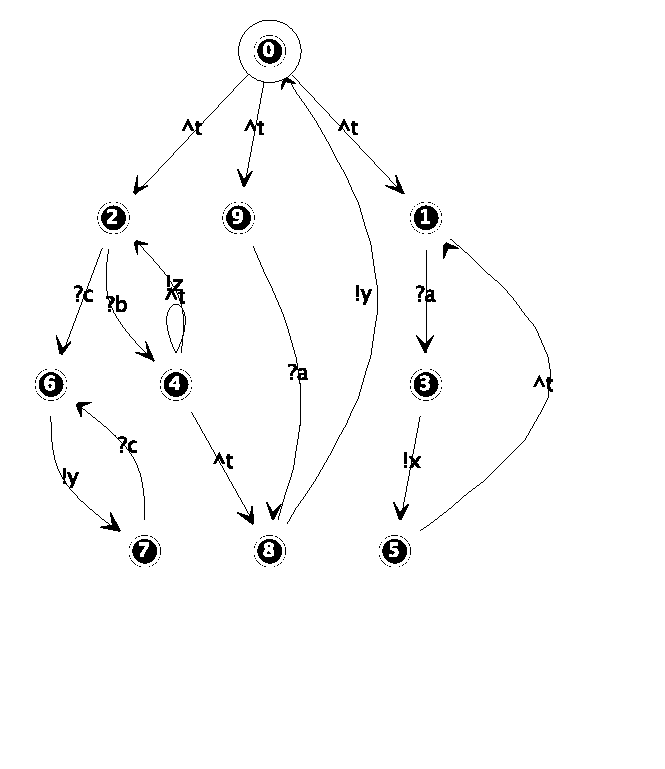
\includegraphics[width=.45\textwidth]{figures/fig-sample-iolts.eps}
    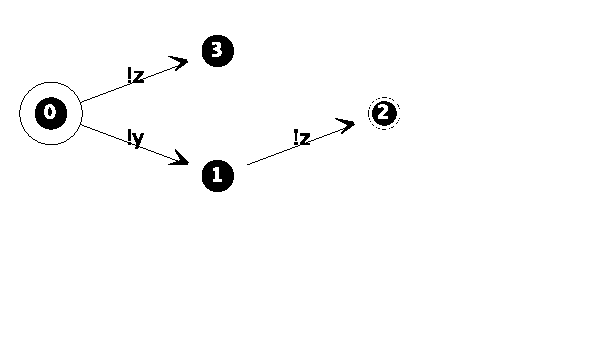
\includegraphics[width=.45\textwidth]{figures/fig-sample-iolts-tp.eps}
    \caption{Sp\'ecification ${\cal S}$ \& Objectif de test ${\cal O }$}
    \label{fig-sample-iolts}
\end{figure}

\begin{figure}[htbp]
    \centering
    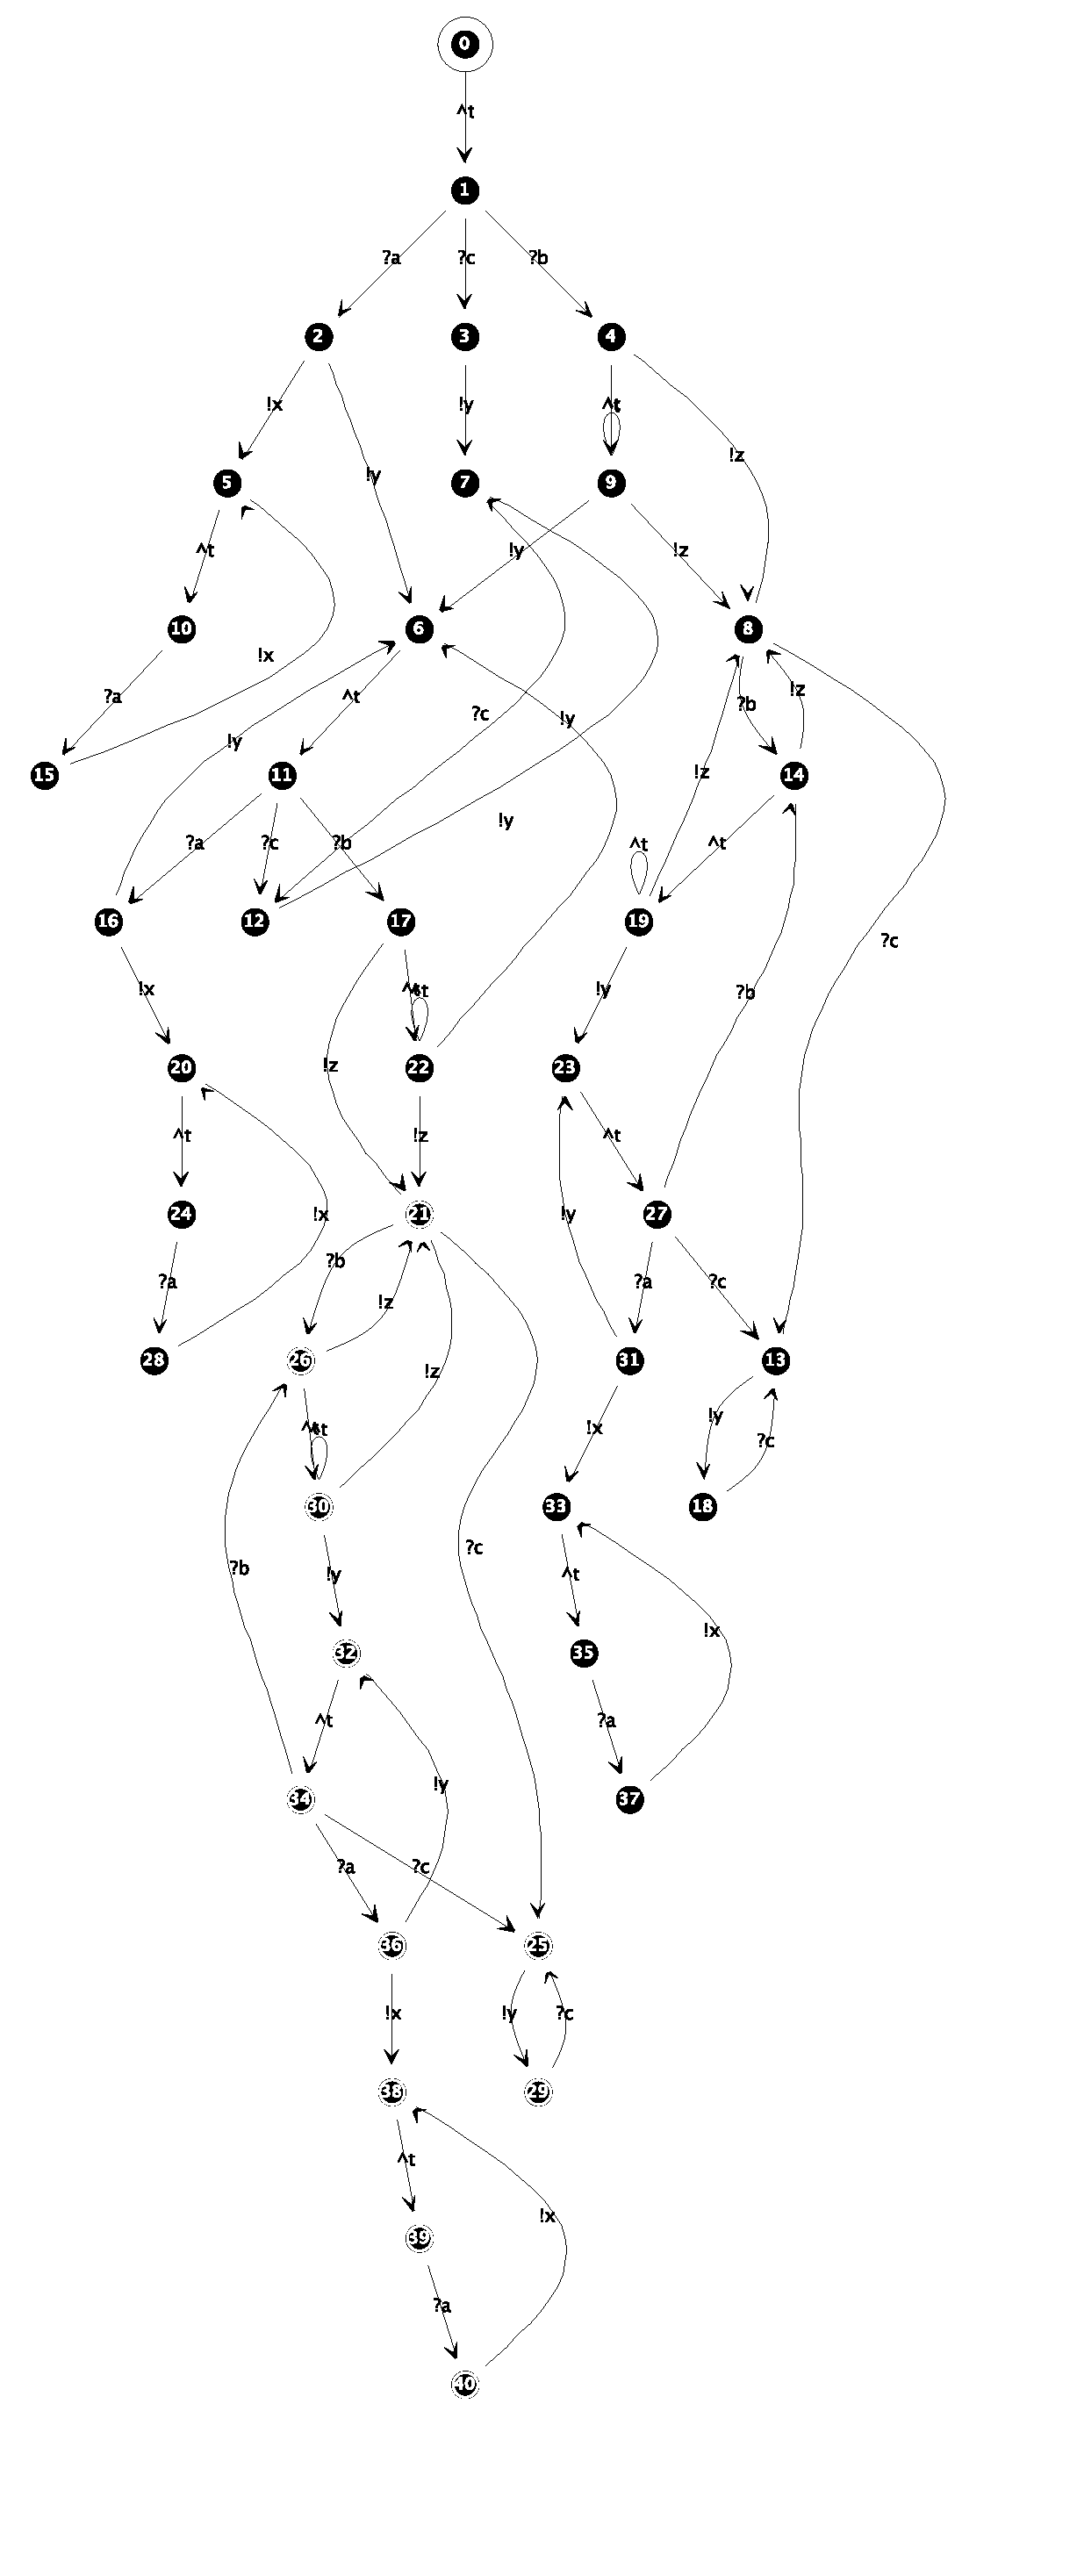
\includegraphics[height=.9\textheight]{figures/fig-sample-iolts-synch.eps}
    \caption{Synchronization ${\cal TP}\|{\cal S}$}
    \label{fig-sample-iolts-synch}
\end{figure}

Sous r\'eserve d'une hypoth\`ese d'\emph{\'equit\'e} --- born\'ee
-- de l'implantation, cette construction permet de s'assurer de la
validit\'e d'une implantation m\^eme dans  les cas de
non-d\'eterminisme de cette derni\`ere. 
La s\'election repose donc sur le choix d'un objectif de
test, solution que l'on retrouve par ailleurs dans d'autres approches
bas\'ees sur ce m\^eme outil\cite{test-pf,stg}.

\subsubsection{\textsc{TorX}}

La g\'en\'eration des cas de tests dans l'outil \textsc{TorX} est
bas\'ee sur les travaux th\'eoriques de
\cite{thtretmans}. Contrairement \`a \textsf{TGV}, la g\'en\'eration et
l'ex\'ecution des cas de test sont effectu\'es concurremment selon
un processus non-d\'eterministe\cite{tgenioq} dit aussi test \emph{online}. La notion d'objectif de test est
absente mais le processus peut \^etre guid\'e par le testeur. 

Le cas de test est un arbre \'etiquet\'e par l'alphabet de la
sp\'ecification auquel on ajoute une transition de \emph{quiescence}
pour g\'erer les comportements de blocage. Il est construit
r\'ecursivement par application non-d\'eterministe des trois
r\`egles suivantes \`a partir d'un \'etat initial $q_0$ :
\begin{enumerate}
  \item l'\'etat courant est un \'etat terminal \texttt{pass} ;
  \item \textbf{une} transition d'entr\'ee \emph{valide} est ajout\'ee \`a
  l'\'etat courant, l'\'etat atteint devient le nouvel \'etat
  courant ;
\item \textbf{toutes} les transitions de sortie possibles plus une transition
  $\delta$ sont ajout\'ees \`a l'\'etat courant, les \'etats
  atteints $q_i$ sont ensuite trait\'es successivement en fonction de
  l'ensemble des transitions \'etiquet\'ees des lettres de sorties
  $o_i\in \Sigma_O$ ou une \'etiquette de quiescence $\delta$ :
  \begin{itemize}
    \item si $o_i\not\in \mathrm{Out}(q)$, l'\'etat est marqu\'e
      \texttt{fail},
    \item si $\delta\not\in \mathrm{Out}(q)$, l'\'etat est marqu\'e
      \texttt{fail},
    \item sinon, l'\'etat atteint devient le nouvel \'etat courant.
  \end{itemize}
\end{enumerate}

\subsection{S\'election de cas de tests pour les \textsf{IOLTS}}
\label{sec:selection-iolts}

Une premi\`ere approche est esquiss\'ee dans \cite{thtretmans},
chapitre 6, o\`u l'auteur propose un cadre th\'eorique au probl\`eme
de la s\'election : une \emph{fonction de valuation} permet d'attribuer \`a
chaque suite de tests $K$ une valeur d\'ependant de son pouvoir de
d\'etection de d\'efauts. Cette fonction est pond\'er\'ee par une partition
de l'espace des \'etats et des erreurs induite par les diff\'erentes
suites de test. Une \emph{fonction de co\^ut} est aussi calcul\'ee
en raison de la taille des suites de tests g\'en\'er\'ees, un
arbitrage \'etant ensuite effectu\'e par le testeur entre ces deux
valeurs. Toutefois, aucune solution concr\`ete n'est propos\'ee pour
le calcul, essentiel, de la fonction de valuation, sauf dans le cas
d'une s\'election bas\'ee sur un objectif de test.

Dans \cite{curgus-analytic-test}, une m\'ethode de s\'election de
cas de tests bas\'ee  sur la d\'efinition d'une \emph{m\'etrique}  de l'espace des
s\'equences de test est propos\'ee. Il est alors possible de
s\'electionner des cas de tests parmi un ensemble donn\'e assurant
une certaine couverture, c'est \`a dire une distance maximale entre
les s\'equences s\'electionn\'ees et l'ensemble des s\'equences
possibles. Le principal inconv\'enient de l'algorithme propos\'e est
qu'il n\'ecessite de partir d'une suite de test, par exemple un
objectif de test. 

Dans \cite{spec-coverage-select,pyhala-test-selection}, la s\'election des cas de test se
fait en utilisant un crit\`ere de couverture de la sp\'ecification,
par exemple la couverture de transitions.  L'algorithme pr\'esent\'e
est similaire \`a l'heuristique de recherche locale pr\'esent\'ee
ci-dessus pour les \textsf{FSM} : l'algorithme cherche \`a maximiser les
transitions couvertes par une recherche des transitions ex\'ecutables
dans son voisinage et effectue un choix al\'eatoire
dans le cas contraire. \cite{kervinen-heuristic} est un raffinement de ces principes :
une fonction d'\'evaluation est associ\'ee \`a chaque transition
courante et \`a chaque \'etat en fonction d'un objectif de
couverture, la valeur d'un \'etat prenant par ailleurs en compte la
valeur des \'etats accessibles \`a partir de
celui-ci jusqu'\`a une certaine profondeur. Diff\'erentes strat\'egies de s\'election sont ensuite
possibles, une strat\'egie dite pessimiste qui consid\`ere que l'\textsf{IUT}
s\'electionne en priorit\'e les transitions avec la plus faible
valuation, une strat\'egie adaptative qui modifie la valeur des
transitions en fonction des transitions d\'ej\`a parcourues.

 \cite{yannakakis-test-opt-games} est une synth\`ese
r\'ecente des approches heuristiques \og modernes\fg pour la
s\'election des cas de test dans les \textsf{IOLTS} : il examine
successivement la mod\'elisation du probl\`eme comme un jeu \`a
deux joueurs, comme un probl\`eme d'optimisation combinatoire et
comme un probl\`eme d'apprentissage supervis\'e. L'auteur rappele un
certain nombre de r\'esultats de d\'ecidabilit\'e et de
complexit\'e sur ces diff\'erentes mod\'elisations. La
mod\'elisation du probl\`eme du test comme un jeu est aussi \`a la
base du test d'\emph{Abstract State Machines} pr\'esent\'e dans
\cite{blass-test-game}. 

Ces diff\'erents travaux s'inspirent de crit\`eres de couverture
utilis\'es dans le test structurel (voir section
\ref{sec:test-structurel})  pour s\'electionner  de mani\`ere
objective et contr\^ol\'ee des suites de tests. Nous pensons que
cette approche est, d'un point de vue pratique, tr\`es
int\'eressante, surtout lorsqu'on cherche \`a int\'egrer dans le
processus de s\'election de cas de tests les donn\'ees. Le chapitre
\ref{cha:test} consacr\'e au test d\'efinira une proc\'edure de s\'election pour les
automates \textsf{FIDL} qui est clairement inspir\'ee  de ces
approches.

\cite{testiodata,gaudel-unitheory} unifient deux formalismes, les \textsf{IOLTS}
et les sp\'ecifications alg\'ebriques dans une m\^eme
d\'emarche. Les sp\'ecifications sont ici des \textsf{IOLTS} 
dont les messages comportent des donn\'ees vues comme des types
alg\'ebriques abstraits. L'ensemble de test exhaustif est construit
\`a partir d'un certain nombre d'hypoth\`eses de testabilit\'e de
l'implantation :
\begin{itemize}
  \item l'implantation est un \textsf{IOLTS} acceptant toujours toutes les
  entr\'ees ;
\item le non-d\'eterminisme est limit\'e par une hypoth\`ese
  d'\'equit\'e born\'ee, c'est \`a dire qu'il existe un entier $n$ tel
  que $n$ ex\'ecutions d'un test assure que tous les choix
  non-d\'eterministes auront \'et\'e faits ;
\item toutes les actions parall\`eles sont ind\'ependantes ;
\item l'implantation dispose d'un \emph{reset} correctement
  implant\'e ;
\item l'\textsf{IOLTS} repr\'esentant l'implantation est fortement convergent :
  il n'existe pas de chemin infini de transitions \'etiquet\'ees par
  un \'ev\'enement interne.
\end{itemize}
L'ensemble de test exhaustif est alors d\'efini comme  l'ensemble des
s\'equences de message de  la sp\'ecification compl\'et\'ees par
 les sorties non autoris\'ees
--- compte tenu de l'\'ev\'enement particulier $\delta$ d\'enotant
l'absence de sorties.  \`A partir de cette d\'efinition, on utilise une
variante de l'algorithme non-d\'eterministe pr\'esent\'e ci-dessus dans la section
consacr\'ee \`a \textsc{ToRX} pour construire des cas de tests
appartenant \`a cet ensemble. 

La construction de la suite concr\`ete de tests d\'epend en fait
d'hypoth\`eses faites sur les param\`etres des messages. \`A partir
d'une description symbolique, on va tout
d'abord d\'efinir une longueur maximale de test (hypoth\`ese de
r\'egularit\'e) permettant de couvrir l'ensemble des \emph{op\'erations}
possibles sur le type des param\`etres, c'est \`a dire tous les
constructeurs du type de donn\'ees en question. Pour am\'eliorer la
couverture des diff\'erents cas, on va d\'eplier les op\'erations
selon les diff\'erentes r\`egles disponibles. Enfin, les valeurs
sont instanci\'ees par r\'esolution des contraintes r\'esultant des
pr\'edicats de gardes pour les diff\'erentes transitions
non-autoris\'ees, c'est \`a dire g\'en\'eralement par
r\'esolution d'une conjonction des n\'egations des diff\'erentes
conditions d'activation de transitions de sorties. 

\subsection{Le test r\'eparti}
\label{sec:le-test-reparti}

\begin{floatingfigure}{.45\textwidth}
    \epsfig{width=.4\textwidth,file=figures/fig-archi-dist-test.eps}
    \caption{Architecture de test r\'eparti}
    \label{fig-archi-dist-test}
\end{floatingfigure}

S'il n'existe pas \`a notre connaissance de \emph{th\'eorie} du test de
composants ou d'architectures logiciels, au sens o\`u nous l'entendons
dans cette th\`ese, il existe par contre de nombreux travaux sur le
probl\`eme du \emph{test r\'eparti}. Dans le test r\'eparti,  le testeur n'est plus  monolithique
mais peut interagir avec le programme test\'e au travers de plusieurs
\emph{points de contr\^ole et d'observation} ou  \textsf{PCO}
\'eventuellement r\'epartis sur un r\'eseau. On remarque que cette 
situation  correspond au probl\`eme du test d'un composant
pouvant offrir et requ\'erir plusieurs interfaces et poss\'eder
plusieurs fl\^ots de contr\^ole  plus ou moins ind\'ependants.

On distinguera le \emph{test r\'eparti coordonn\'e}, dans lequel les
testeurs  ont la possibilit\'e de se synchroniser entre eux du \emph{test r\'eparti pur}
dans lequel les testeurs ne disposent pas de cette facilit\'e. La
figure \ref{fig-archi-dist-test} repr\'esente sch\'ematiquement ces
architectures de test : le trait pointill\'e entre les testeurs
n'existe pas dans une architecture de test r\'eparti pur.

\subsubsection{Test r\'eparti pur}

Le test r\'eparti pur a \'et\'e \'etudi\'e en particulier dans
\cite{luo-tgen-dist,sarikaya-proto-test,hierons-check-synch} pour ce
qui concerne le mod\`ele des (E)\textsf{FSM}. Nous ne connaissons pas
d'\'etude concernant ce probl\`eme appliqu\'e au test d'\textsf{IOLTS}.
Dans cette configuration, des d\'efauts peuvent appara\^{\i}tre de par
la nature partielle des observations et du contr\^ole que chaque
testeur a de l'implantation sous test : il peut ne pas y avoir de lien
direct entre une entr\'ee sur un \textsf{PCO} donn\'ee et les sorties sur ce
PCO, ce qui revient \`a dire qu'on ne peut pas toujours conna\^{\i}tre
l'\'etat global du syst\`eme test\'e \`a partir de ses \'etats
locaux, un probl\`eme classique de l'algorithmique distribu\'ee. 

Dans tous le cas, le syst\`eme est repr\'esent\'e par un \textsf{FSM} dont
l'alphabet d'entr\'ee et de sortie est partitionn\'e entre les
diff\'erents \textsf{PCO} du syst\`eme, les transitions peuvent donc mettre
en \oe uvre des ports diff\'erents pour l'entr\'ee et la sortie. 

\cite{luo-tgen-dist,sarikaya-proto-test} cherchent \`a construire une
s\'equence de test de type \emph{tour de transition} qui sera dite
\emph{synchronisable} : une s\'equence est synchronisable si toutes
les paires de transitions  de la
s\'equence sont synchronisables c'est \`a dire si l'on peut toujours
les ordonner localement sur un ou plusieurs ports. Il existe bien s\^ur des cas o\`u une telle s\'equence
n'existe pas, ce qui signifie que l'on ne peut pas toujours
v\'erifier la conformit\'e d'une \textsf{IUT} dans une architecture
distribu\'ee pure. 

Sur le m\^eme mod\`ele,
\cite{hierons-check-synch} cherche \`a construire une s\'equence de
v\'erification selon l'algorithme \textsf{UIO}. Un probl\`eme connexe \`a la
synchronisation est celui des d\'ecalages de sortie, dans le cas
o\`u une sortie correcte observable sur un port peut appara\^{\i}tre
sur deux transitions cons\'ecutives dont l'une n'est pas d\'ependante
d'une entr\'ee sur le m\^eme port. La m\'ethode pr\'esent\'ee
est de construire des s\'equences d'UIO synchronisables pour chacun
des ports et chacun des \'etats du syst\`eme en transformant le
graphe de la sp\'ecification initiale de mani\`ere \`a identifier
les probl\`emes de synchronisation.  Comme pr\'ec\'edemment, la
possibilit\'e de construire un ensemble de test d\'epend fortement
de la structure initiale de la sp\'ecification.

\subsubsection{Test r\'eparti synchronis\'e}

Le cas du test r\'eparti synchronis\'e a \'et\'e comparativement
plus \'etudi\'e car il correspond \`a une situation plus favorable
pour le testeur et  r\'ealiste dans un contexte de test en cours
de d\'eveloppement. Cette architecture est similaire au test
centralis\'e puisque les testeurs  
ont toute latitude pour reconstruire en communiquant un \'etat global
\`a partir de leurs \'etats locaux.

Dans \cite{cacciari-dist-test}, ce probl\`eme est \'etudi\'e dans
l'univers des \textsf{FSM} et le principal r\'esultat est un algorithme
permettant de synchroniser des testeurs locaux avec un nombre garanti
minimal de messages \'echang\'es.

Dans le monde des \textsf{IOLTS},
\cite{ulrich-concur-testing} introduit une
s\'emantique concurrente non-entrelac\'ee pour l'ordonnancement
des messages entre les diff\'erents testeurs. La construction de
s\'equences de test est
bas\'ee sur la construction de r\'eseaux de Petri \`a partir de
sp\'ecifications \textsf{IOLTS} puis sur le \emph{d\'epliage} du r\'eseau global
obtenu \`a partir des sp\'ecifications locales de mani\`ere \`a
obtenir un graphe dirig\'e acyclique des pr\'efixes
d'\'ev\'enements d\'ependants les uns des autres. Le d\'epliage
s'arr\^ete lorsque des configurations d'\'ev\'enements d\'ej\`a
atteintes sont rencontr\'ees, les \'ev\'enements concurrents
introduisant des points de branchement dans le d\'epliage. Cette
construction est applicable uniquement en l'absence d'interblocage
 dans la sp\'ecification, une propri\'et\'e qui peut
\'eventuellement \^etre v\'erifi\'ee par
\emph{model-checking}. Le graphe de d\'ependance d\'epli\'e peut
ensuite \^etre utilis\'e pour g\'en\'erer des s\'equences de
test de conformit\'e qui sont ensuites projet\'ees sur les testeurs
locaux pour ex\'ecution. 

Ce m\^eme principe est appliqu\'e dans \cite{jard-synth-dist-test}
pour \'etendre les principes de la g\'en\'eration de cas de tests
de \textsf{TGV} au cas des testeurs r\'epartis. Le formalisme utilis\'e est
l\'eg\`erement diff\'erent et plus complexe que dans \cite{ulrich-concur-testing} mais
surtout le principe du d\'epliage des \'ev\'enements concurrents
est dirig\'e par l'\emph{objectif de test}. De plus, les
d\'ependances entre \'ev\'enements sur des testeurs diff\'erents
sont contr\^ol\'ees par l'insertion de messages de synchronisation
entre testeurs comme dans \cite{cacciari-dist-test}. Notons que dans
tous les cas cit\'es, il est n\'ecessaire de construire la
sp\'ecification globale de l'IUT.

La formalisation de la notion de testeur r\'eparti et des relations
d'implantation correspondantes est d\'etaill\'ee dans
\cite{heerink-miots-test,heerink-factor-miots}. L'auteur d\'efinit un
\emph{MIOTS}, c'est \`a dire un \textsf{IOLTS} dont les alphabets d'entr\'ee
et de sortie sont partitionn\'es sur un ensemble de canaux --- les
PCO ---, et une relation d'implantation \textbf{mioco} similaire \`a
\textbf{ioco} --- un pr\'eordre sur les ensembles de traces-refus
---- mais param\'etr\'ee par la partition des alphabets. 

Bien que nous ayons remarqu\'e l'absence d'outils th\'eoriques
propres au test de composants architecturaux,
\cite{composition-testing-ioco} s'est int\'eress\'e au probl\`eme
du test de \emph{composants} en g\'en\'eral dans le cadre de la
relation \textbf{ioco} et des \textsf{IOLTS}. Il montre que sous l'hypoth\`ese
de certaines restrictions, il n'est pas n\'ecessaire de retester
le r\'esultat de la composition de deux composants qui sont
\textbf{ioco} conformes \`a leur sp\'ecification respectives. La
composition est ici entendu au sens d'un produit de synchronisation
des alphabets internes aux deux composants suivi d'une projection.

\section{Test structurel \& Crit\`eres de couverture}
\label{sec:test-structurel}

Bien qu'il ne constitue pas l'objet principal de notre \'etude, cette
section pr\'esente une synth\`ese des techniques de test dit
structurel. Premi\`erement, parce qu'il s'agit des techniques les
plus courantes dans le domaine du test de logiciel. Et deuxi\`emement
parce que l'on constate une convergence entre les deux approches, les notions de crit\`eres de test et de couverture \'etant
de plus en plus utilis\'e pour s\'electionner des cas de tests
fonctionnels (\emph{cf.} section \ref{sec:selection-iolts}). 

Un crit\`ere de couverture est un objectif de
test qui est bas\'e sur une mesure de couverture d'un certain nombre
de traits de l'analogue de l'objet test\'e, g\'en\'eralement le
code source. C'est historiquement un concept
essentiel et qui a donn\'e lieu \`a un nombre consid\'erable de
travaux th\'eoriques et pratiques sur la d\'efinition de crit\`eres
pertinents --- on dira aussi \emph{ad\'equat} --- et
sur les comparaisons entre crit\`eres. C'est aussi bien souvent le
seul crit\`ere objectif dont on dispose en pratique pour d\'efinir
un objectif de test. 

\cite{goodenough-test-selection} est certainement un des articles les
plus cit\'es dans le domaine du test : il fonde l'ensemble de la
th\'eorie de la s\'election des cas de tests en introduisant les
concepts fondamentaux de \emph{fiabilit\'e} d'une suite de test et
d'\emph{ad\'equation}  par rapport \`a un crit\`ere. 

Une suite de tests pour un programme sur un certain domaine
d'entr\'ee est dite \emph{fiable} si lorsque la suite de tests ne
produit aucune panne, le programme ne contient aucune erreur. 
Une suite de tests pour un programme sur un certain domaine
d'entr\'ee  est dite \emph{ad\'equate} si la suite de tests est capable
de d\'etecter tous les programmes produisant des sorties incorrectes
pour tous les \'el\'ements du domaine d'entr\'ee. On remarquera que
ces notions sont fortement similaires aux propri\'et\'es attendues
des suites de tests fonctionnelles.

\subsubsection{Typologie des crit\`eres}

Les crit\`eres de couverture peuvent \^etre bas\'es sur le graphe
de contr\^ole de l'analogue de l'\textsf{IUT}, sur le graphe de flots de
donn\'ees, sur la structure de l'espace d'entr\'ee et de l'espace de
sortie, ou une combinaison quelconque de l'un de ces crit\`eres.
\cite{zhu-coverage} propose une classification des crit\`eres de test
et des analyses de leur efficacit\'e, c'est \`a dire de leur
capacit\'e \`a d\'etecter des erreurs. Ces analyses se basent en
particulier sur les travaux de \cite{faultdetect} qui d\'efinissent
une relation de subsomption entre ensembles de crit\`eres de test. 

\begin{figure}
    \centering
\begin{lstlisting}[linewidth=.45\textwidth,language=Java]
    public boolean verifyUIO(Map m) {
        if(m.size() != states().size())
            return false;
        List[] words = new List[m.size()];
        words = (List[]) 
             m.values().toArray(words);
        final int len = words.length;
        for(int i=0;i<len;i++)
            for(int j=i+1;j<len;j++)
                if(words[i].equals(words[j]))
                    return false;
        return true;
    }
\end{lstlisting}
    
    \caption{Code source Java de la figure \ref{fig-sample-control}}
    \label{fig-source-sample-control}
\end{figure}

Les crit\`eres bas\'es sur la structure du fl\^ot de contr\^ole du
programme vont de la couverture des instructions ---
\emph{all-statements} --- \`a la couverture des chemins ---
\emph{all-paths}, en passant par la couverture du nombre
cyclomatique, la couverture des branches --- \emph{all-edges}, la
couverture des conditions et d\'ecisions --- \emph{Multiple Condition
Decision Coverage} ou MCDC.

La figure \ref{fig-sample-control} est une repr\'esentation du
graphe de contr\^ole d'une m\'ethode \textsf{Java} obtenu \`a
partir du code octet. Ce graphe correspond au code source de la figure
\ref{fig-source-sample-control} qui est une m\'ethode qui v\'erifie
pour un \textsf{FSM} que chaque s\'equence associ\'e
\`a chaque \'etat est bien une s\'equence \textsf{UIO} (voir
ci-dessus \ref{sec:la-methode-uio}).

\begin{figure}[htbp]
    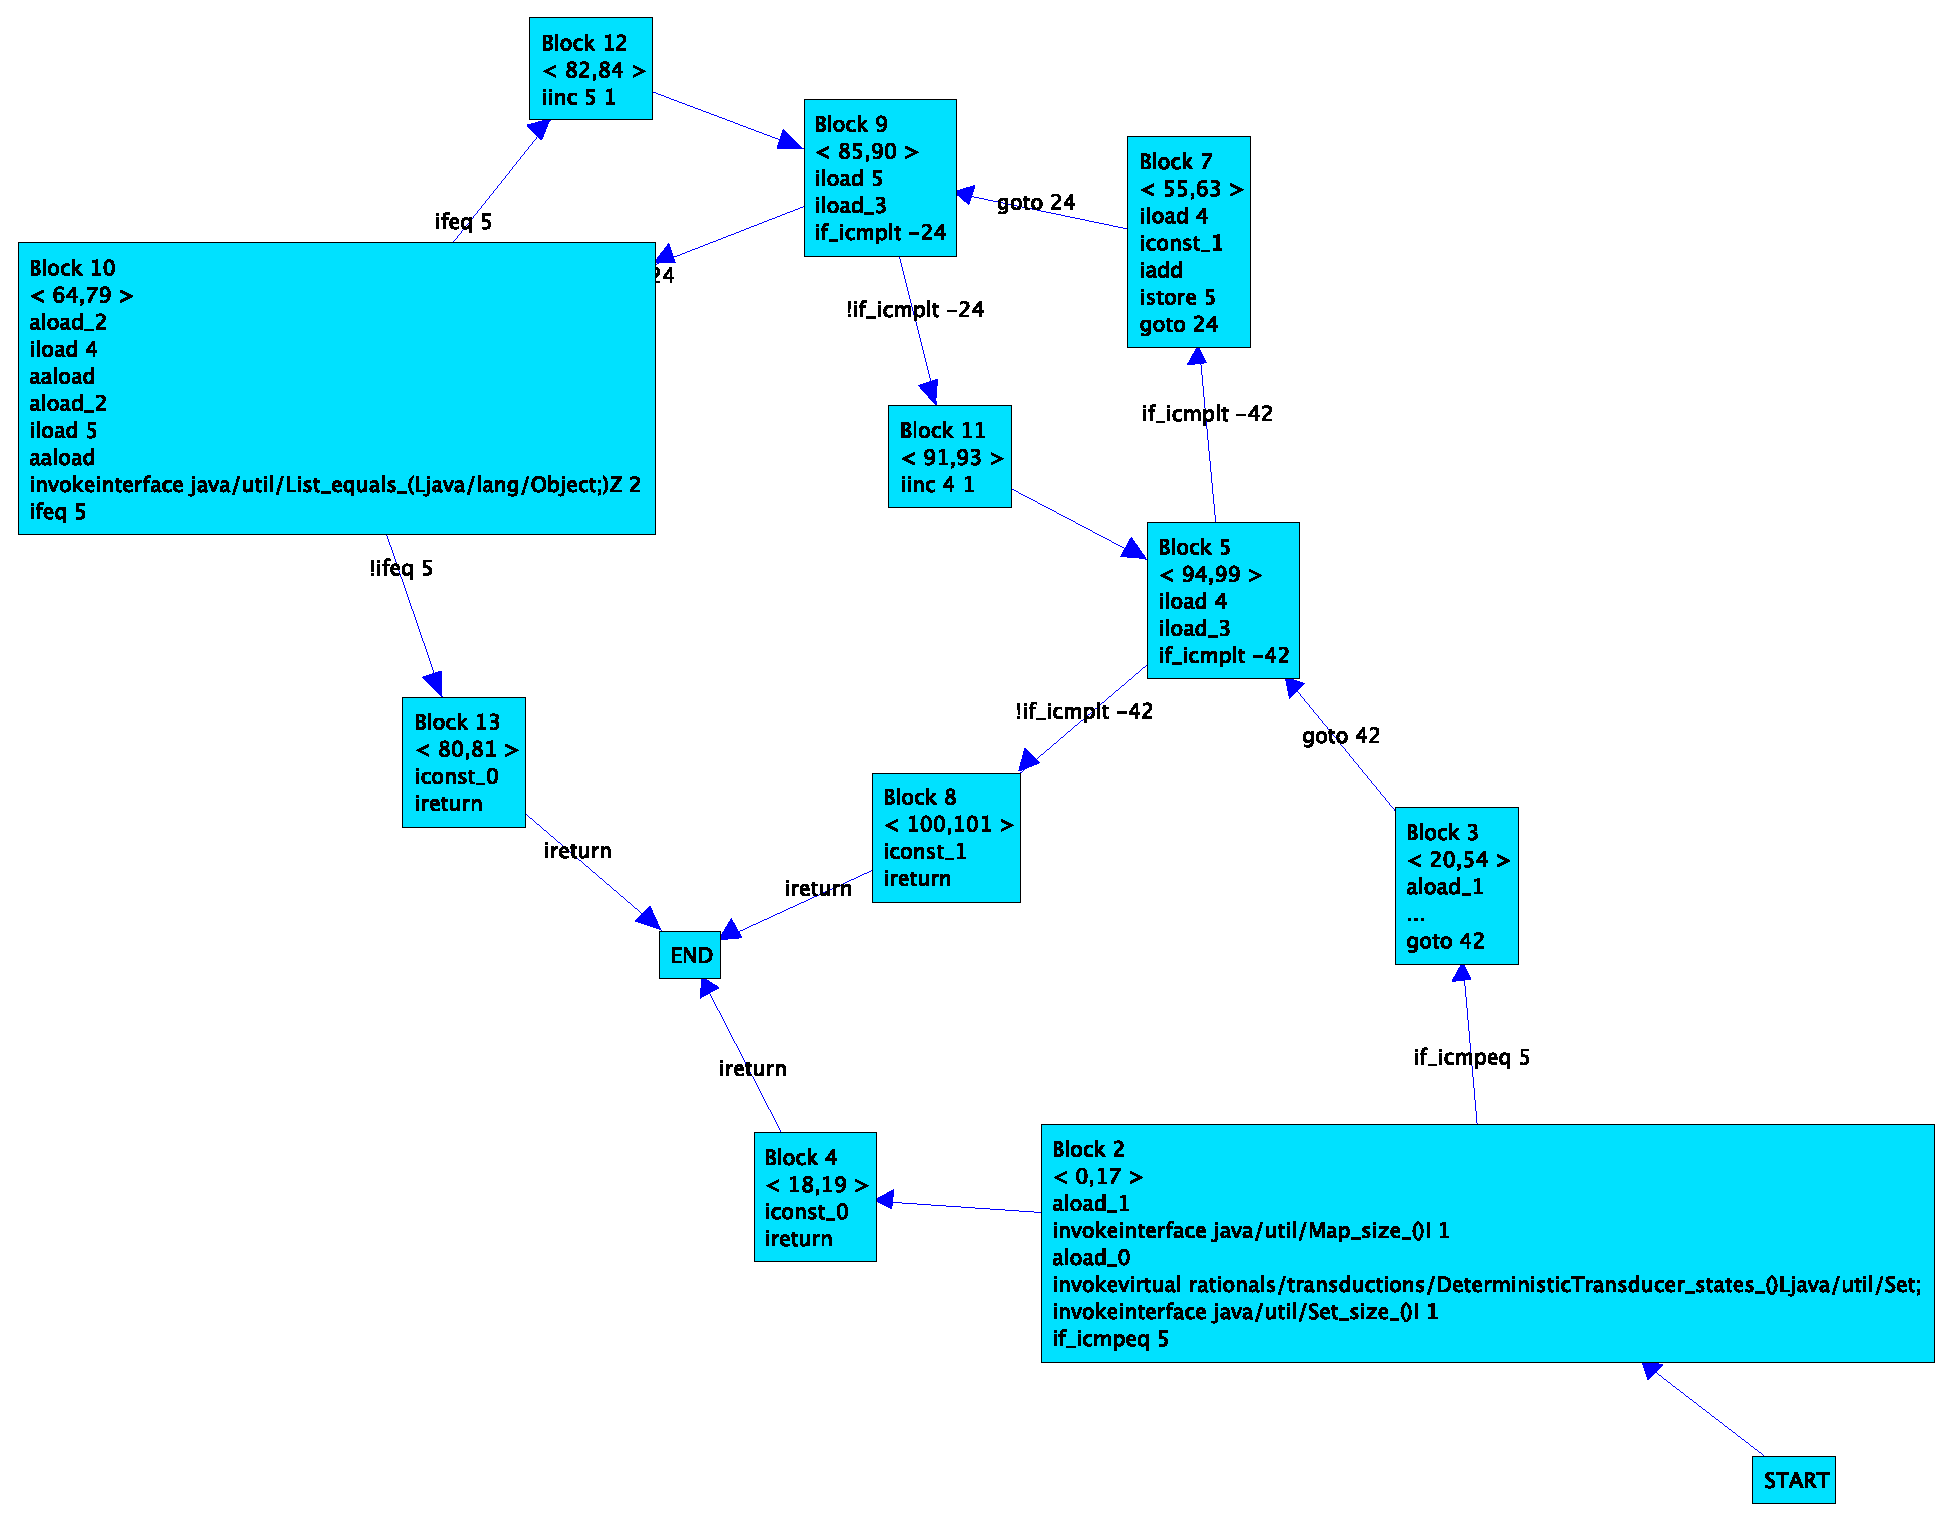
\includegraphics[width=\textwidth]{figures/fig-sample-control.eps}
    \caption{Exemple de graphe de contr\^ole}
    \label{fig-sample-control}
\end{figure}

\`A partir du graphe pr\'esent\'e, on peut donc d\'efinir en
fonction de diff\'erents crit\`eres de couvertures des
suites de tests qui sont des ensembles de chemins dans le
graphe de contr\^ole. Il restera pour chacune de ces s\'equences
\`a d\'efinir les valeurs de variables permettant de r\'ealiser
effectivement la s\'equence choisi, ce qui est un probl\`eme souvent
ardu. 

Par exemple, l'ensemble $\{(2,3,5,7,9,11,5,7,9,10,12,9,10,13), (2,4),
(2,3,5,8)\}$ est potentiellement ad\'equat pour les crit\`eres \emph{tous-les-n\oe uds} et
\emph{tous-les-arcs} du graphe de contr\^ole de  la figure
\ref{fig-source-sample-control}. Il reste \`a montrer qu'un certain
ensemble des valeurs des variables d'entr\'ee permet de sensibiliser
ces chemins.

Les crit\`eres bas\'es sur le flot de donn\'ees s'int\'eressent
\`a la couverture des relations entre la d\'efinition d'une
variable et son utilisation. Une hi\'erarchie de 
crit\`eres bas\'ee sur la notion de chemin \emph{def-use} est aussi construite. La figure
\ref{fig-sample-data} est une repr\'esentation d'un graphe de
flot de donn\'ees simplifi\'e pour le graphe de contr\^ole
\ref{fig-sample-control}. Les n\oe uds sont des utilisations ou des
d\'efinitions de variables --- marqu\'ees \textsf{Use i} ou
\textsf{Def i} --- et les arcs sont une extension des arcs du graphe
de contr\^ole permettant de relier chaque n\oe ud. 

Nous n'avons pas ici distingu\'e les n\oe uds de type
\emph{p-use} --- utilisation d'une variable pour un pr\'edicat de
branchement conditionnel --- des n\oe uds \emph{c-use} --- utilisation
pour une instruction, un appel .... \cite{vincenzi-covtest-java} est une proposition d'outil et de
m\'ethode pour le test de couverture de fl\^ot de contr\^ole et de
donn\'ees pour programmes \textsf{Java}. Comme dans les exemples
pr\'esent\'es figures \ref{fig-sample-control} et
\ref{fig-sample-data}, le principe est d'extraire ces graphes du
\emph{code-octet} repr\'esentant un programme \textsf{Java}.

\begin{figure}[htbp]
    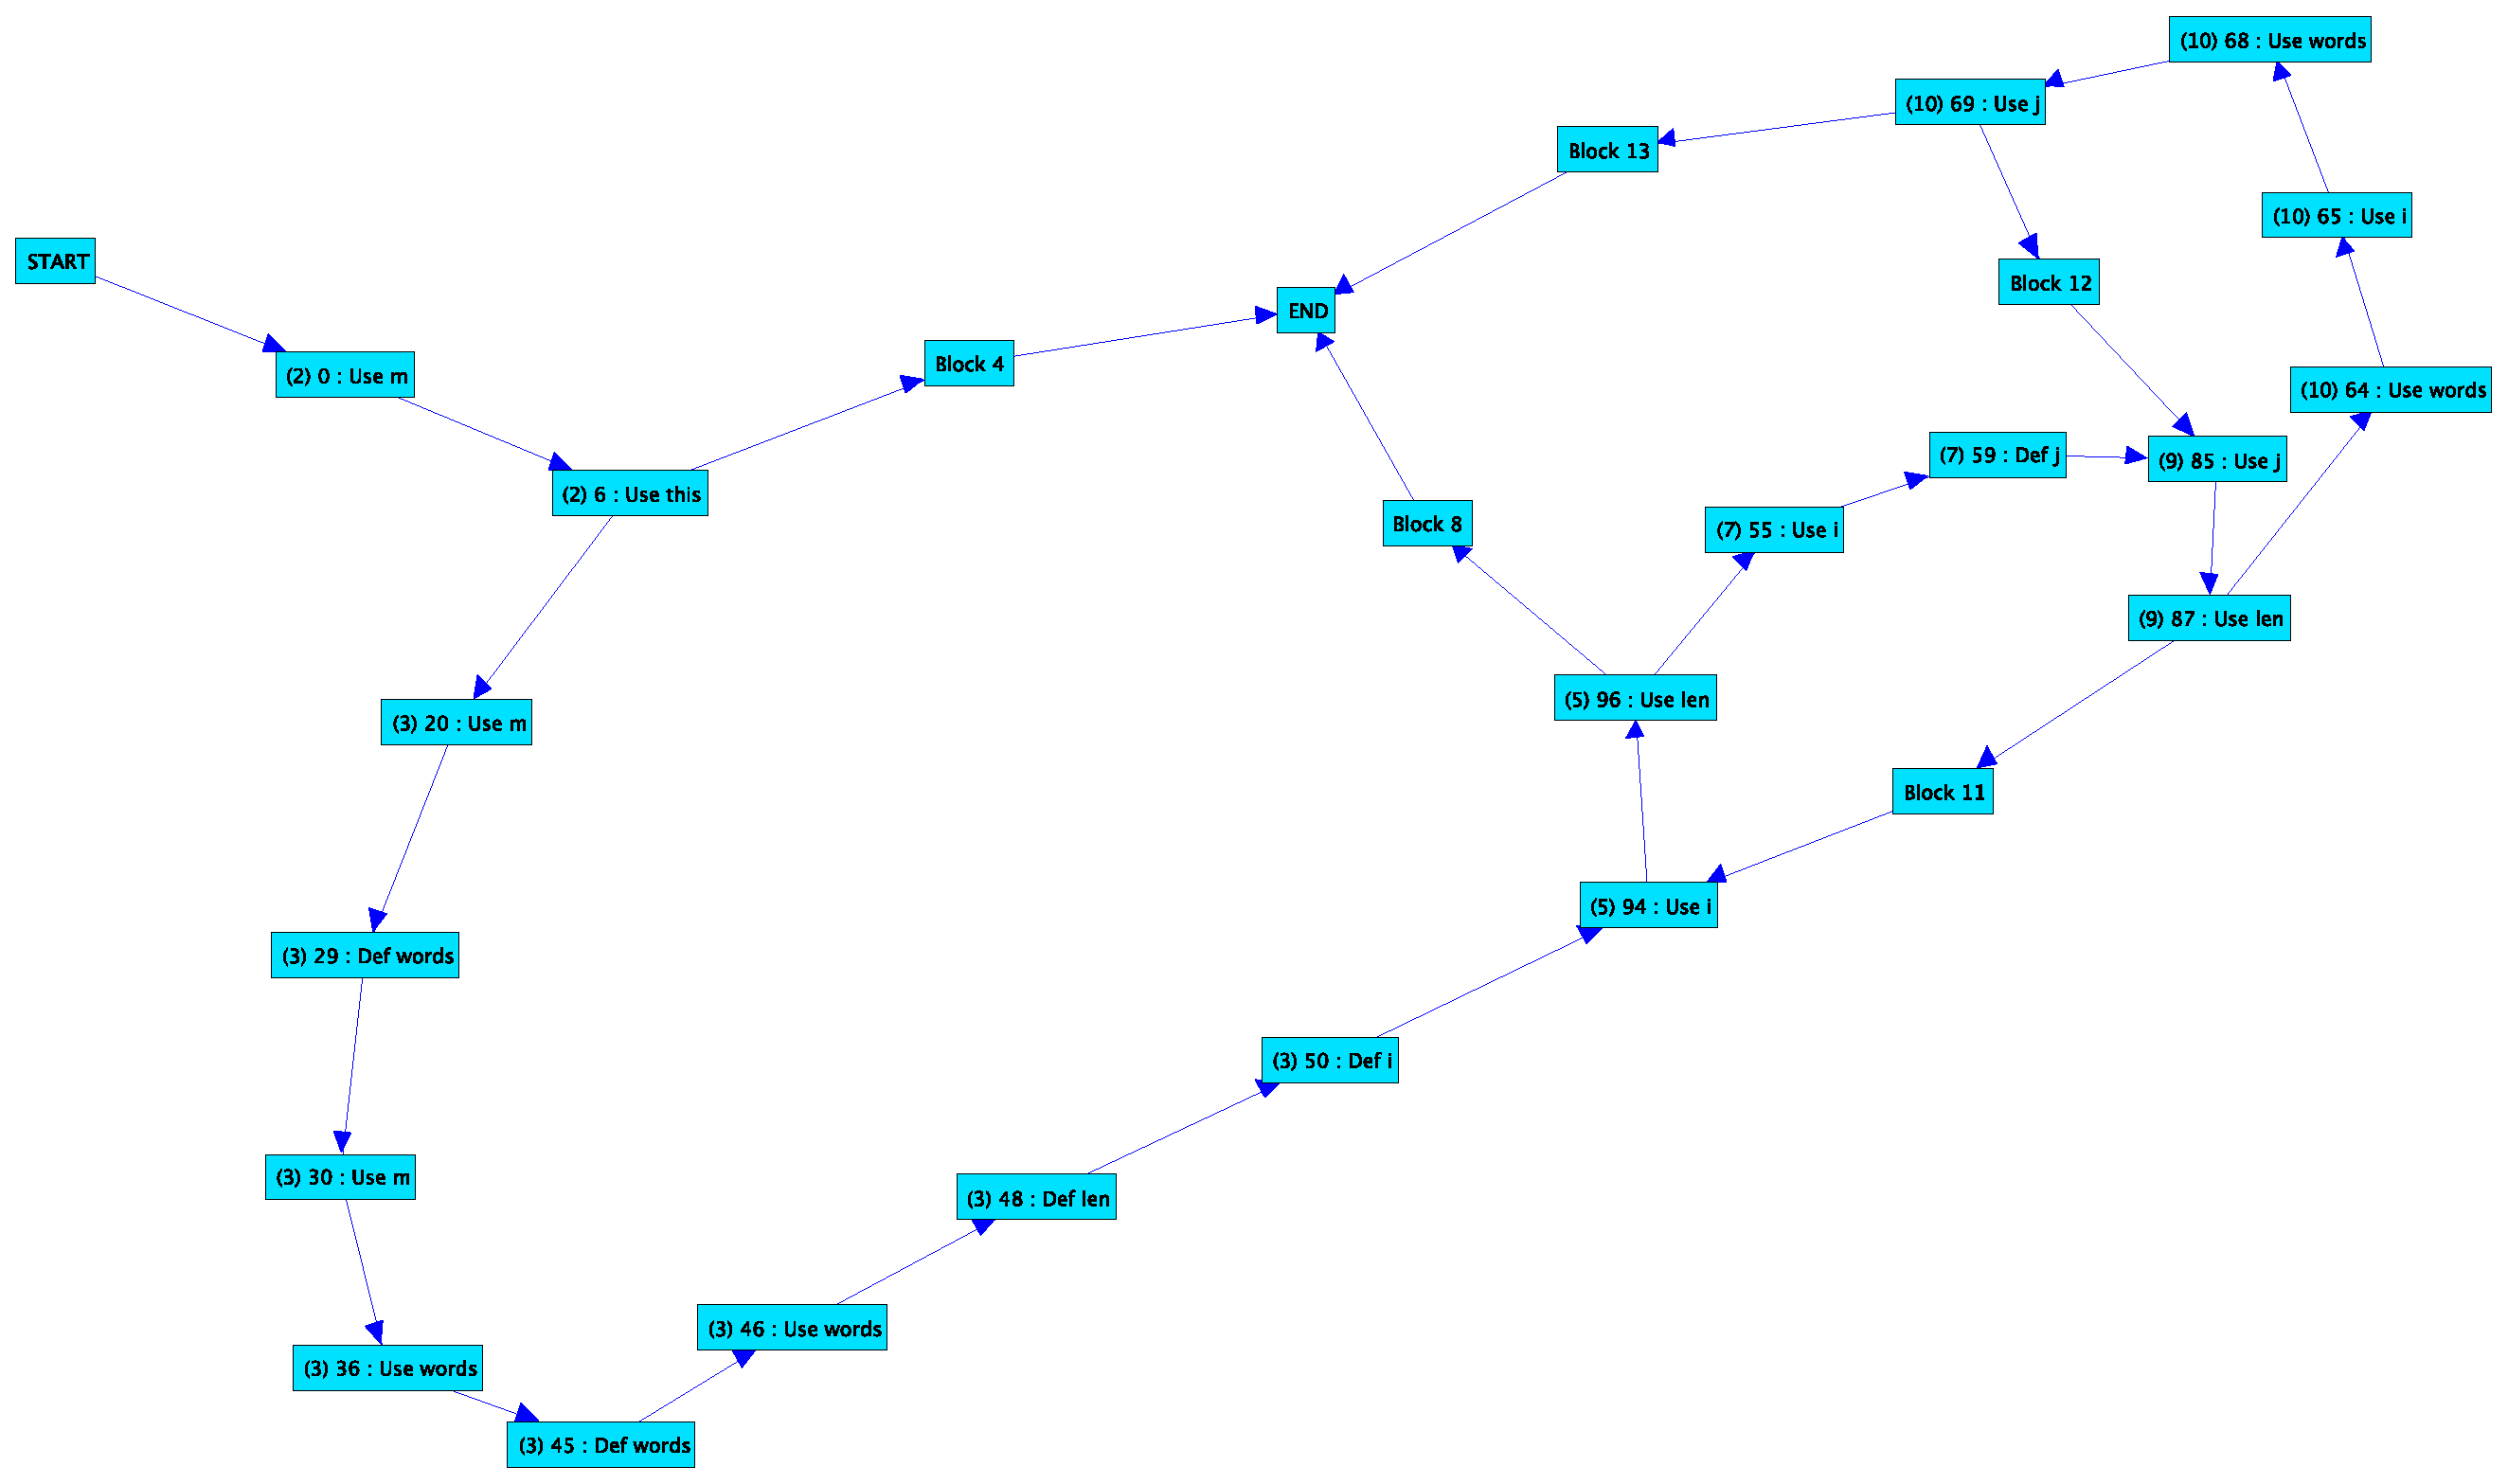
\includegraphics[width=\textwidth]{figures/fig-sample-data.eps}
    \caption{Exemple de graphe de flot de donn\'ees}
    \label{fig-sample-data}
\end{figure}

Le probl\`eme principal li\'e \`a l'utilisation de crit\`eres de
ce genre consiste bien \'evidemment \`a construire un jeu de tests
permettant de respecter le crit\`ere ce qui n'est pas toujours
possible et est m\^eme ind\'ecidable dans le cas g\'en\'eral.
La figure \ref{fig-hierarchie-couv} pr\'esente une vue partielle de
cette hi\'erarchie des crit\`eres de test pour quelques crit\`eres courants.

\begin{figure}[htbp]
    \centering
    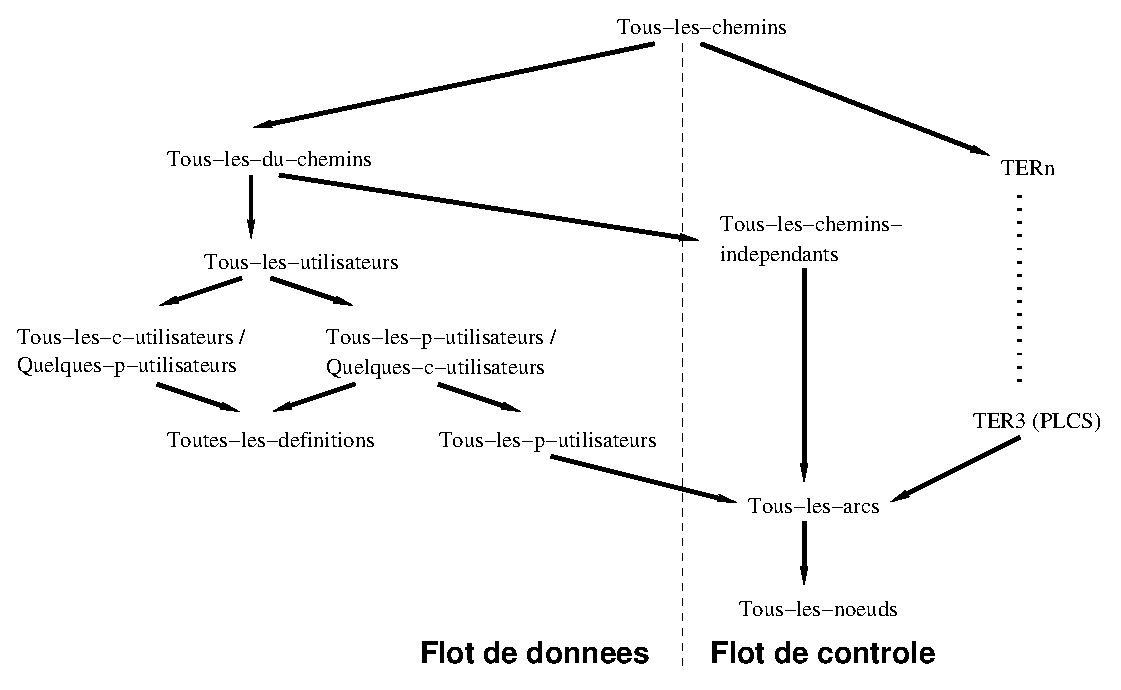
\includegraphics[width=\textwidth] {figures/hiertest.eps}
    \caption{Hi\'erarchie usuelle des crit\`eres de couverture}
    \label{fig-hierarchie-couv}
\end{figure}

Ce  probl\`eme  de \emph{sensibilisation} des chemins d'ex\'ecution
possible du programme a \'et\'e d\'ej\`a abord\'e dans
\cite{boyer-select} comme une forme d\'eriv\'ee de la preuve
automatique de th\'eor\`eme. Le principe de \texttt{SELECT} est de
r\'ealiser une ex\'ecution symbolique du programme test\'e pour
construire des ensembles des chemins d'ex\'ecution ayant la forme de
pr\'edicats sur les variables du programme. Les syst\`emes de
contraintes ainsi construits sont ensuite r\'esolus pour fournir des
valeurs d'entr\'ee permettant de sensibiliser chaque chemin. Ce
principe a \'et\'e repris dans \cite{gotlieb-clp-test} et dans
l'outil \textsf{InKa} d\'eriv\'e de ces travaux, en utilisant en syst\`eme
de r\'esolution de contraintes.

On peut aussi utiliser d'autres solutions algorithmiques pour
rechercher des valeurs permettant de sensibiliser un chemin
particulier comme par exemple l'algorithme g\'en\'etique de
\cite{testgenetic} : un vecteur de valeurs d'entr\'ee est
optimis\'e en fonction d'un objectif --- chemin ou \'etat --- et du
nombre de pr\'edicats que le vecteur de valeurs permet de satisfaire
--- fonction de \emph{fitness}.  \cite{tdgen-survey} est une \'etude
des diff\'erentes techniques de recherche heuristiques utilis\'ees
pour la d\'ecouverte de donn\'ees permettant de sensibiliser des
chemins dans un graphe de contr\^ole.

\subsubsection{Analyse de domaine}

Pour s\'electionner les cas de tests, on peut aussi s'int\'eresser
aux caract\'eristiques de l'espace d'entr\'ee ou de sortie du
programme et d\'efinir un objectif en fonction de celui-ci et d'une
\emph{partition}  du domaine en sous-domaines permettant de
sensibiliser tel ou tel chemin ou de valider tel crit\`ere. Une tactique usuelle consiste \`a s'int\'eresser
aux valeurs limites de chaque sous-domaine, sous l'hypoth\`ese que ce
sont ces valeurs qui seront le plus pathog\`enes. Dans le cas des
domaines num\'eriques entiers,  cette strat\'egie permet
classiquement de d\'etecter des erreurs d'utilisation de relations
entre valeurs, un $\leq$ se transformant par exemple en un
$<$. \cite{kosmatov-boundary-issre04} pr\'esente une formalisation de
ce crit\`ere au cas de sp\'ecifications formelles de type \textsf{Z}
ou \textsf{B}. Les partitions de domaines sont d\'eduites des
pr\'edicats sur les variables de la sp\'ecification et r\'esolues
par approximation dans un domaine continu --- par exemple les r\'eels
--- puis retransform\'ees dans le domaine --- discret
d'origine. 
La notion de partitionnement de domaine est aussi sous-jacente dans
les hypoth\`eses de r\'egularit\'e et d'uniformit\'e introduites
dans \cite{gaudel}.

\subsection{S\'election statistique \& al\'eatoire}

Dans la premi\`ere partie de ce chapitre, nous avons introduit la
notion de \emph{profil op\'erationnel} comme un outil d'aide \`a la
s\'election des tests dans le test dit syst\`eme. Un profil
op\'erationnel est simplement une distribution probabiliste de
l'espace d'entr\'ee de l'\textsf{IUT}. Une tactique de test \'evidente
consiste donc \`a \'echantillonner cette espace d'entr\'ee pour
l'utiliser comme donn\'ee de test et \`a
induire des lois  statistiques une fiabilit\'e du logiciel en
fonction des r\'esultats du test. \cite{thprobtest} propose de formaliser le test
probabiliste fonctionnel, de mani\`ere similaire \`a
l'ing\'enierie de la fiabilit\'e, en calculant \`a partir d'un
\'echantillonage des valeurs de l'espace d'entr\'ee une
probabilit\'e de correction --- pour des tests r\'eussis --- en
fonction d'une marge d'erreur et d'un intervalle de confiance. 

\cite{thevenod-stat-test} d\'efinit une notion de qualit\'e de
test en fonction d'un crit\`ere de test et de la taille de la suite
de tests s\'electionn\'ee par \'echantillonage sur une distribution
de l'espace d'entr\'ee construite en fonction du crit\`ere de
couverture \`a atteindre. Il ne s'agit plus ici d'un
profil op\'erationnel correspondant \`a un usage attendu de l'IUT
mais d'un \emph{profil de test} sp\'ecifiquement construit en
fonction d'un objectif pr\'ed\'efini et permettant d'\'evaluer la
qualit\'e du r\'esultat produit de mani\`ere statistique. Bien
s\^ur, la fiabilit\'e globale du test r\'ealis\'e reste
d\'ependante de la confiance que l'on place dans le crit\`ere choisi,
avec cette diff\'erence par rapport au cas d\'eterministe que les
cas de tests sont s\'electionn\'es al\'eatoirement et donc sans
le biais  d'une s\'election arbitraire. Cette technique est
d\'evelopp\'ee dans \cite{gouraud-issre04}, en utilisant des
techniques de g\'en\'eration al\'eatoire de structures
combinatoires, pour le test statistique bas\'e sur des
sp\'ecifications prenant la forme de graphes.

Lorsque la distribution est uniforme, on a alors un \emph{test
  al\'eatoire}. \cite{thevenod-structtest,ntafos-comparison} montrent
exp\'erimentalement qu'il n'est pas forc\'ement l'approche la moins efficace pour la
d\'etection des erreurs.

\subsection{Test mutationnel}

Le test mutationnel --- \emph{mutation testing} en anglais ---
constitue une
technique indirecte pour s\'electionner une suite de test pertinente.
Cette technique a \'et\'e introduite dans
\cite{demillo-mutation}. Son principe est d'\'evaluer la
fiabilit\'e de la suite de test par rapport \`a un \emph{mod\`ele
  de faute} : 
\begin{itemize}
  \item on d\'efinit pour un langage ou un format binaire donn\'e un
    ensemble d'\emph{op\'erateurs de mutations} atomiques : inversion
    de relations binaires, changements de variables, transformations
    d'op\'erateurs arithm\'etiques, modifications de constantes en
    variables, ... Ces op\'erateurs de mutation repr\'esentent  des
    erreurs courantes que peut introduire un \emph{programmeur
      comp\'etent} dans un logiciel et constituent donc un mod\`ele
    des fautes que la suite de test va rechercher ;
  \item on applique ces op\'erateurs de mani\`ere \og
    syst\'ematique~\fg sur le logiciel test\'e produisant ainsi des
    \emph{mutants}, c'est \`a dire des versions proches du logiciel
    original mais g\'en\'eralement incorrectes. Chaque mutant diverge de son parent par
    une seule op\'eration de mutation selon le principe du couplage
    des erreurs : une suite de test r\'ev\'elant des erreurs simples
    sera capable de r\'ev\'eler des erreurs complexes. Autrement
    dit, les erreurs complexes sont issues de plusieurs erreurs simples
    (voir \cite{offutt-coupling} pour une discussion exp\'erimentale de
    la question). Le probl\`eme des mutants \'equivalents  est loin d'\^etre trivial mais
    est n\'eglig\'e en pratique ;
  \item on \'ecrit ou enrichit une suite de tests \emph{tuant}
    le maximum de mutant, c'est \`a dire que lorsqu'elle est
    ex\'ecut\'ee sur les mutants, elle r\'ev\`ele qu'ils sont
    incorrects en produisant \'echec du test ;
\item le \emph{score de mutation} de la suite de tests est \'egal au
  nombre de mutants tu\'es sur le nombre total de mutants non-\'equivalents.
\end{itemize}
Ce score de mutation est une mesure de la qualit\'e de la suite de
tests et donc de la qualit\'e du logiciel : si le logiciel  passe la
suite de tests dont le score de mutation est \'elev\'e, c'est donc
qu'il ne contient pas les fautes inject\'ees par le test de
mutation. Implicitement, cette m\'ethode se base sur deux
hypoth\`eses :
\begin{description}
  \item[Hypoth\`ese du programmeur comp\'etent] : le logiciel
  test\'e est \emph{a priori} presque correct et les erreurs de
  programmation sont simples ;
\item[Hypoth\`ese du couplage] : les erreurs complexes sont des
  suites d'erreurs simples.
\end{description}

On voit bien que la fiabilit\'e de cette approche  d\'epend du choix
des op\'erateurs de mutation et de leur ad\'equation avec les erreurs
susceptibles de se produire r\'eellement, ainsi que du nombre et de
la r\'epartition des mutants g\'en\'er\'es. Ce dernier point la
rend d'ailleurs tr\`es co\^uteuse en temps d'ex\'ecution et de
r\'ealisation des tests. Dans \cite{these-baudry}, cette approche est
utilis\'ee coupl\'ee avec un algorithme g\'en\'etique pour
optimiser des suites de tests.

Le test mutationnel a une litt\'erature relativement abondante et a
donn\'e lieu \`a la cr\'eation d'une faune vari\'ee
d'op\'erateurs de mutations, en particulier dans le cadre des
langages \`a objets. Cette technique est tr\`es
utilis\'ee pour comparer des  m\'ethodes de s\'election de cas de
test entre elles. 

\section{Discussion}

On a vu que le test logiciel, m\^eme restreint au seul cas du test de
syst\`emes \`a \'etats-transitions, offre un champ
extr\^emement vaste de travaux qui se sont toutefois essentiellement
concentr\'es dans deux directions : d'une part la s\'election
efficiente de suites de tests dans le cas des \textsf{FSM}, d'autre part la
d\'efinition de relations de conformit\'e pertinentes dans le
domaine des \textsf{IOLTS}. 

Nous avons aussi vu que le probl\`eme de la s\'election des cas de
test se ramenait essentiellement au probl\`eme de la d\'efinition
d'un \emph{objectif de test}, au sens large du terme, d\'ependant des
artefacts \`a la disposition du testeur, et qu'il existait un nombre
tr\`es importants de crit\`eres heuristiques difficilement
comparables entre eux.

\subsection{Test bas\'e sur les mod\`eles}

Nous nous sommes concentr\'es dans l'exposition de cet \'etat de
l'art sur des m\'ethodes \emph{primitives} de test. Ces m\'ethodes
constituent la  base d'autres m\'ethodes utilisant des mod\`eles
de plus haut niveau tels que les diagrammes \textsf{UML} ou, plus
rarement, les \textsf{ADL}.

Il existe une litt\'erature importante consacr\'ee \`a
l'application de ces m\'ethodes au cas de diagrammes \textsf{UML} et
plus particuli\`erement des
Statecharts\cite{jezequel-msc-testd,umlaut,umlinttest,offutt,tdgen-state,testselectstatecharts,scollo-archi-test}.
La question de tests d'int\'egration et de leur ordonnancement \`a
partir de mod\`eles UML est abord\'ee dans \cite{umlinttest} et
\cite{jeron-integ-regr-ootest}. 
\cite{test-pf} est une approche bas\'ee sur les cas d'utilisation et
les contraintes associ\'ees. \`A partir d'un diagramme  de cas
d'utilisations enrichi de pr\'edicats et  de variables, et des
d\'ependances entre cas d'utilisations, on construit
un diagramme d'\'etats finis qui est inject\'e dans \textsf{TGV}
pour produire une suite de tests
syst\`emes. \cite{briand-uml-systesting} a une approche similaire
bas\'ee sur l'utilisation de contraintes \textsf{OCL}. 

\cite{muccini-archi-test} propose une m\'ethode d'extraction de cas
de tests unitaires \`a partir d'une description d'architecture dont
le comportement est mod\'elis\'e sous forme de \textsf{LTS}. Ce
travail est dans l'id\'ee proche de notre d\'emarche : il s'agit de
construire des tests de composants \`a partir d'une sp\'ecification
d'architecture. Dans le d\'etail, les m\'ethodes diff\`erent : le
test n'est pas ici conduit de mani\`ere syst\'ematique mais \`a
partir de la d\'efinition d'un \emph{objectif de test}, le crit\`ere
de s\'election choisi est bas\'e sur la complexit\'e de
\textsc{McCabe}\cite{mccabe-complexity-testing}, les tests abstraits d\'eriv\'es doivent \^etre
manuellement \og traduits\fg en tests ex\'ecutables en fonction du
composant test\'e. 
\cite{tool-ccm-test,ccmtesting} pr\'esentent une architecture et un
outil pour le test de composants \textsf{CCM}. La question du
probl\`eme de la s\'election des cas de tests n'est toutefois pas
abord\'ee. \cite{cavalli-corba-iscc} est une application aux objets
\textsf{CORBA} de l'algorithme \emph{Hit-Or-Jump} pr\'esent\'e \`a
la section \ref{sec:test-fsm-heuristic}. 

\subsection{Analyse}

\cite{lai-prototest-survey} souligne la distance qui
existe entre la foultitude de mod\`eles et d'algorithmes produits par
le monde universitaire et l'\'etat concret des pratiques dans
l'industrie :
\begin{quote}
    \og [...] this state-of-the-art research is not necessarily
    state-of-the-practice. Academic methods are seldom employed in
    industry. [...] There is not much progress in the use of test
    sequence generation techniques for practical testing of
    communication networks. \fg
\end{quote}
La port\'ee  de cette affirmation doit toutefois \^etre
mod\'er\'ee par le fait que l'auteur n'envisage qu'une classe de
syst\`emes de transitions dans son \'etude, les \textsf{FSM}. Il n'en reste
pas moins vrai que l'activit\'e du test dans le monde industriel est
encore largement \og manuelle\fg.
La situation est identique dans le monde des services logiciels comme on l'a vu au chapitre
\ref{cha:proc-de-devol}. 

Les notions d'\'equivalence dans les FSM et les IOLTS sont
fondamentalement diff\'erentes. Dans le premier cas, on a une
\'equivalence entre des \emph{fonctions} : le \textsf{FSM} est un
transducteur calculant une fonction \`a partir de param\`etres
d'entr\'ee. Le but du test de conformit\'e de \textsf{FSM} est de
v\'erifier ce calcul en parcourant l'espace des valeurs du
param\`etre d'entr\'ee qui est ici un \emph{langage}. Dans le second
cas, on v\'erifie une \'equivalence entre des \emph{langages}. Les
suite de tests ont donc des statuts et des structures diff\'erentes :
un ensemble de s\'equences d'entr\'ee d'une part, un ensemble de
mots du langage d'autre part. Et le processus de test est bien s\^ur
diff\'erent : sensibilisation du FSM d'une part, synchronisation des
deux langages d'autre part.

Le panorama que nous avons fait dans ce chapitre nous permet de mieux
nous orienter dans l'approche choisie. On voit clairement que notre
objectif est similaire \`a celui du test de conformit\'e
r\'eparti pour des syst\`emes de transitions \`a entr\'ee-sortie (section
\ref{sec:le-test-reparti}). Ces travaux s'appuient sur les relations de conformit\'e
d\'efinies \`a la section \ref{sec:test-de-lts}. Ces
relations,  et en particulier la relation
\textbf{ioco}, ne sont toutefois pas satisfaisantes dans notre
contexte : elles ne tiennent pas compte de
la nature \emph{contractuelle} des sp\'ecifications de composants que
nous utilisons ni de l'asym\'etrie existant dans les
composants entre les interfaces requises et les interfaces fournies. 
 
Par ailleurs, notre approche de la mod\'elisation des composants est fond\'ee sur les automates et
la th\'eorie des langages. Il est donc naturel que nous choisissions
d'exprimer la notion de conformit\'e en termes d'une relation
d'\'equivalence sur des langages et par cons\'equent que les tests
permettant de v\'erifier cette relation soient r\'ealis\'es sous la
forme d'un produit de synchronisation entre les langages.

%%% Local Variables: 
%%% mode: latex
%%% TeX-master: "these"
%%% End: 
